%%%%%%%%%%%%%%%%%%%%%%%%%%%%%%%%%%%%%%%%%%%%%%%%%%%%%%%%%%%%%%%%%%%%%%
% Missing Semester MIT Adaptation - Well not that much any longer, 
% we took an entirely new road by now. 

% Primary Author: Prof. Dr.-Ing. Mark Schutera
% Based on Tufte-style layout

% TODOs
% - Buy one of the standardwerke from the introduction and sprinkle ideas on the lecture and excercises.
% - Sprinkle ideas on infinity all over the place (there is this book)
% - Run index generation on the whole thing
% - Check and add references where needed.
% - Check chapters for NTH nice to haves and decide on whether to do them.

% - Think about how to integrate the code better into the lecture. The notebooks did not work as intended 
% - Maybe think playground and sandboxes instead? For short hands-on experiences? 

% Think about flipped classroom and record excercises, or probeklausuren and old exams. 
% - maybe make this a recorded script as well? 

%%%%%%%%%%%%%%%%%%%%%%%%%%%%%%%%%%%%%%%%%%%%%%%%%%%%%%%%%%%%%%%%%%%%%%

% Auszug Modulhandbuch. Numerische Methoden (12 H Präsenzzeit):
% - Fehleranalyse: Kondition, Rundungsfehler, Stabilität
% - Numerische Integration
% - Fixpunktiterationen
% - Newton-Verfahren
% Optional: Interpolation & Approximation (Polynominterpolation, Splines): 
% Polynominterpolation (Lagrange und Hermite), Splines (B-Splines), Fourierreihen



\makeindex
%%%%%%%%%%%%%%%%%%%%%%%%%%%%%%%%%%%%%%%%%%%%%%%%%%%%%%%%%%%%%%%%%%%%%%

\documentclass{../sharedAssets/tufte}

%%
% Book metadata
\title{Numerical Methods}
\author[\defaultauthor]{\defaultauthor}
\publisher[\defaultpublisher]{\defaultpublisher}
\renewcommand{\notesdir}{notes_numerischemethoden}

% Load optional fonts
\loadoptionalfonts

% Additional packages
\usepackage{pifont}
\usepackage{amsmath}
\usepackage{soul}
\usepackage{textcase}
\usepackage{enumitem}
\usepackage{tikz}
\usepackage{pgfplots}
\pgfplotsset{compat=1.18}
\usepackage{float}
\usepackage{algorithm}
\usepackage{algpseudocode}

\begin{document}



\makestandardfrontmatter
% Dedication
% Alternative quotes:
\makededication{\openepigraph{"An infinitely accurate approximation \\is no longer an approximation."}{Probably someone smart}}
\tableofcontents


% Introduction
\makeintroduction{%
    \newthought{Numerical Methods} are essential for solving mathematical problems that cannot be addressed analytically. 
    This course will cover fundamental concepts, error analysis, problem conditioning, stability, and various numerical techniques to equip you with the 
    skills needed to implement reliable and efficient algorithms in scientific computing and engineering applications.
}
     
\newthought{This course will teach you} everything you need to know to become proficient with numerical methods, and how to put them to
good use in machine learning, data science, and engineering contexts.

\makephilosophy

\iffalse
\marginnote{\newthought{Contact} \\\url{blochinger@dhbw-ravensburg.de}\\
\newthought{Source} \\ \url{https://www.economicon.de/repository/index.html}}
His thoughts on Numerical Methods have been of great help and carry ideas which infused this lecture.
\fi

%\newthought{Acknowledgments} to Prof. Dr. Daniel Blochinger at DHBW Ravensburg, 
%who handed over this course to me in my first Semester as a Professor.




%% Start the main matter
\mainmatter
\authorinrectoheader


% ----------------------------------------------------------------------

% Modulhandbuch:
% - Fehleranalyse: Kondition, Rundungsfehler, Stabilität
% - Numerische Integration
% - Fixpunktiterationen
% - Newton-Verfahren
% - Optional: Interpolation & Approximation (Polynominterpolation, Splines):
%             Polynominterpolation (Lagrange und Hermite), Splines (B-Splines), Fourierreihen



\input{chapters/1_introduction.tex}
\input{chapters/2_floatingpointarithmetics.tex}
\input{chapters/3_erroranalysis.tex}
\index{Newton method}
\chapter{Newton Methods}
\printchapterversion{4_newton_methods}
\newthought{A Step in the Right direction.}

% TODO
% Think about introducing fixpoint iterations as a family first, then introduce Newton as a specific method within that family.

% TODO
% Introduce the convergence order of the Secant method: super-linear with
% p = phi = (1 + sqrt(5)) / 2 ~ 1.618 (the golden ratio). Sits between linear
% (e.g. bisection) and quadratic (Newton). Worth contrasting explicitly with
% Newton's p = 2, so students can reason about iteration counts to reach a
% given tolerance.



% ==============================================================================================
% INTRODUCTION BLOCK

\section{The Why}

\index{local information}
\index{derivative}
\newthought{In the previous chapter}, 
we characterized numerical methods with conditioning, stability, consistency, and convergence.
But our brute-force grid search is fundamentally limited: it explores the solution space blindly, 
requiring $O(N^d)$ evaluations for $N$ grid points in $d$ dimensions.

\newthought{The key insight} is deceptively simple: instead of asking "what is the value here?" at every grid point, we also ask "which way should I go next?".
The function's slope, its derivative, tells us the direction towards the solution.
This transforms search fundamentally.

\newthought{Understanding these methods} allows us to:
\begin{itemize}
    \item Use local information to make sophisticated steps instead of brute-force searches
    \item Achieve faster and more optimal convergence.
\end{itemize}

\index{gradient descent}
\newthought{In Machine Learning and Deep Learning,} Newton's method simplified to first order is also known as 
gradient descent. One could argue that the entire field of deep learning is built on the idea of using 
local gradient information to navigate toward minima in a high-dimensional loss landscape, 
to train models that are optimized towards specific objectives.

\marginnote{\newthought{Backpropagation} is of course as vital to distribute gradient information through the layers of a neural network, but the core optimization step is still a form of gradient-based navigation.}








\newpage
\subsection{Hands On Experience}

For starters let's get an intuitive feel for the power of using local information.
We compare grid search with Newton's method on the same sine function from Chapter 3, 
but now we're finding where it crosses zero: $\sin(x) = 0$ on the interval $[2.5, 4]$ 
(the solution is near $\pi \approx 3.14159$). 



\begin{figure}[h]
    \centering
    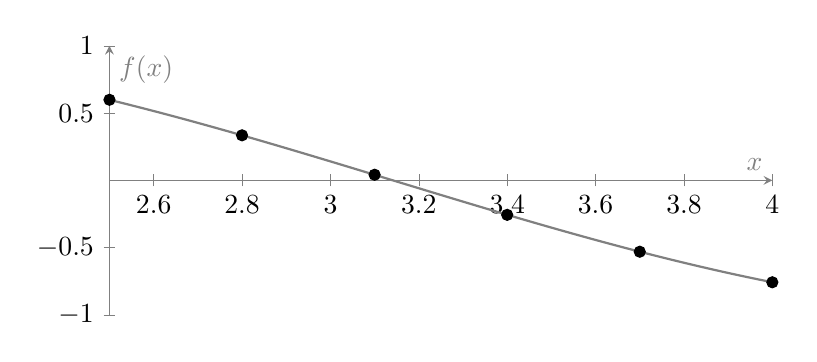
\begin{tikzpicture}
        \begin{axis}[
              width=10cm,
              height=5cm,
              axis x line=middle,
              axis y line=middle,
              xlabel={$x$},
              ylabel={$f(x)$},
              domain=2.5:4,
              samples=100,
              ymin=-1, ymax=1,
              xmin=2.5, xmax=4,
              legend style={at={(0.5,-0.2)},anchor=north},
              tick style={gray},
              label style={gray},
              axis line style={gray},
        ]
            % Continuous curve
        \addplot[gray, thick, smooth] {sin(deg(x))};
        % Discretized points for h=0.3
        \addplot[black, only marks, mark=*] coordinates {
            (2.5, 0.599)
            (2.8, 0.335)
            (3.1, 0.042)
            (3.4, -0.256)
            (3.7, -0.530)
            (4.0, -0.757)
        };
        \end{axis}
    \end{tikzpicture}
    \caption{Continuous curve $f(x) = \sin(x)$ on $[2.5,4]$, and discretized points with step size $h=0.3$.}
    \label{fig:newton_sine_gridsearch}
\end{figure}

\newthought{Grid search} on $[2.5, 4]$ with step $h = 0.3$ evaluates blindly:
\begin{align*}
    f(2.5) &\approx 0.599 \\
    f(2.8) &\approx 0.335 \\
    f(3.1) &\approx 0.042 \quad \leftarrow \text{closest to zero} \\
    f(3.4) &\approx -0.256 \\
    f(3.7) &\approx -0.530 \\
    f(4.0) &\approx -0.757
\end{align*}
We found $x \approx 3.1$ with 6 evaluations, with an error $|3.1 - \pi| \approx 0.042$.

\newthought{Newton's method} has an adaptive approach to search. 
At every point we evaluate the function and its derivative, and use this local information to make a step towards the solution.

\begin{figure}[h]
    \centering
    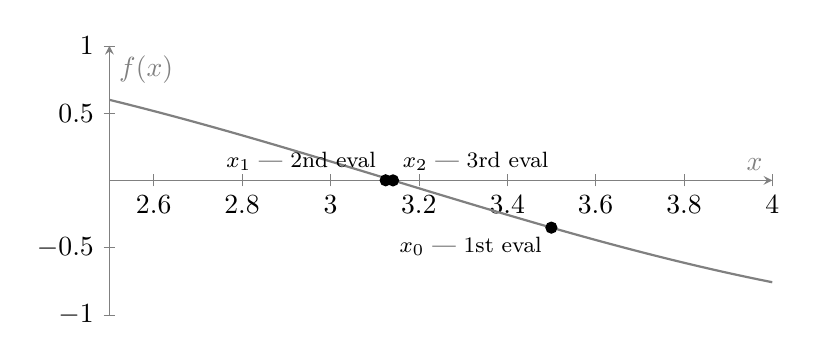
\begin{tikzpicture}
        \begin{axis}[
              width=10cm,
              height=5cm,
              axis x line=middle,
              axis y line=middle,
              xlabel={$x$},
              ylabel={$f(x)$},
              domain=2.5:4,
              samples=100,
              ymin=-1, ymax=1,
              xmin=2.5, xmax=4,
              legend style={at={(0.5,-0.2)},anchor=north},
              tick style={gray},
              label style={gray},
              axis line style={gray},
        ]
            % Continuous curve
        \addplot[gray, thick, smooth] {sin(deg(x))};
        % Newton iteration points
        \addplot[black, only marks, mark=*] coordinates {
            (3.5, -0.351)
            (3.125, 0.0008)
            (3.14159, 0.0)
        };
        % Iteration annotations
        \node[below left, font=\footnotesize] at (axis cs:3.5, -0.351) {$x_0$ | 1st eval};
        \node[above left, font=\footnotesize] at (axis cs:3.125, 0.0008) {$x_1$ | 2nd eval};
        \node[above right, font=\footnotesize] at (axis cs:3.14159, 0.0) {$x_2$ | 3rd eval};
        \end{axis}
    \end{tikzpicture}
    \caption{Newton's method iterations: starting from $x_0=3.5$, converging rapidly to $\pi \approx 3.14159$.}
    \label{fig:newton_sine_iteration}
\end{figure}

\marginnote{\newthought{We pay for this sophistication} with more hyperparameters that we need to determine and more 
complex computations (derivative evaluation and division), but we gain in convergence speed.}


\newthought{Derivative as source of local information} $f'(x) = \cos(x)$ 
gives the slope of the tangent at a given point. 
There are multiple ways to use this information to derive the direction and the size of the next step: We for sure want to move in the direction where the function decreases, then we could take a step with fixed size, or we could make the step size proportional to the derivative.
Let's just take the next guess where the tangent crosses zero for now - which is the solution to the linear approximation of $f$ at $x_n$. 


Starting at $x_0 = 3.5$:
\begin{align*}
    x_1 &= x_0 - \frac{\sin(x_0)}{\cos(x_0)}\\
    &= 3.5 - \frac{-0.351}{-0.936} \\
    &= 3.5 - 0.375 \\
    &= 3.125 \\
    x_2 &= 3.125 - \frac{\sin(3.125)}{\cos(3.125)} \\
    &= 3.125 - \frac{0.0008}{-0.9999} \\
    &\approx 3.14159 \\
    x_3 &\approx 3.14159 \\
    \text{and } \sin(3.14159) &\approx 0
\end{align*}

After just 2 iterations, to be fair this means 4 function/derivative evaluations, we have $x \approx 3.14159$ with error $< 10^{-5}$.
The derivative told us where to look way more efficiently than we have been used to.


\vspace{2.5em}
\newthought{The Learning Objectives} of this chapter aim at providing you with the abilities to:
\begin{itemize}
    \item Derive and apply Newton-Raphson iteration for root finding in 1D
    \item Derive and understnad the Taylor expansion and its role in Newton's method
    \item Analyze convergence rates and failure modes for Newton's method
    \item Understand and apply the Secant method when derivatives are unavailable
\end{itemize}

\marginnote{\newthought{"Newton-Rhapson"} because Isaac Newton came up with the general idea, 
while Joseph Raphson simplified the approach into a practical iterative method.}



% ==============================================================================================
% MAIN THEORY BLOCK
\newpage
\section{Newton-Raphson and Taylor Expansion}
\index{Newton-Raphson}
\index{linear approximation}

\begin{figure}[h]
    \centering
    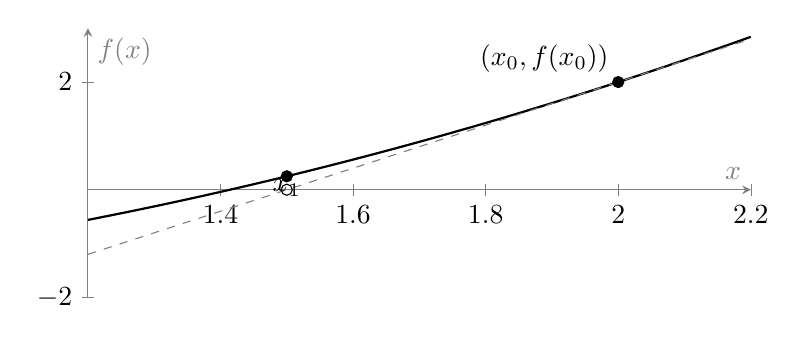
\begin{tikzpicture}
        \begin{axis}[
            width=10cm,
            height=5cm,
            axis x line=middle,
            axis y line=middle,
            xlabel={$x$},
            ylabel={$f(x)$},
            domain=1.2:2.2,
            samples=100,
            ymin=-2, ymax=3,
            xmin=1.2, xmax=2.2,
            tick style={gray},
            label style={gray},
            axis line style={gray},
        ]
        % The function f(x) = x^2 - 2
        \addplot[black, thick, smooth] {x^2 - 2};

        % Tangent line at x=2: f(2)=2, f'(2)=4, tangent: y-2=4(x-2) => y=4x-6
        \addplot[gray, dashed, domain=1.2:2.2] {4*x - 6};

        % Point at x_0 = 2
        \addplot[black, only marks, mark=*, mark size=2pt] coordinates {(2, 2)};
        \node[above left] at (axis cs:2,2) {$(x_0, f(x_0))$};

        % Point where tangent crosses x-axis: x = 1.5
        \addplot[black, only marks, mark=o, mark size=2pt] coordinates {(1.5, 0)};
        \node[above] at (axis cs:1.5,-0.3) {$x_1$};

        % Solid dot on curve at x = 1.5 and f(x)
        \addplot[black, only marks, mark=*, mark size=2pt] coordinates {(1.5, 0.25)};

        \end{axis}
    \end{tikzpicture}
    \caption{Newton's method geometric intuition: For $f(x) = x^2 - 2$, the tangent line at $(x_0, f(x_0))$ intersects the $x$-axis at $x_1$, our next approximation.}
    \label{fig:newton_geometric}
\end{figure}

\vspace{1em}

\newthought{Above} you can see the geometric intuition behind Newton's method for a single iteration. 
Let's formalize the approach of finding $x^*$ such that $f(x^*) = 0$.

\marginnote{\newthought{Note:} This linear approximation is the first-order Taylor expansion of $f$ around $x_n$. We'll return to Taylor expansions later when we study accuracy and approximation formally.}

\newthought{The linear approximation is effectively} given as:
\begin{equation}
    f(x) \approx  f'(x_n) \cdot (x - x_n) \quad \text{for } x \text{ close to } x_n + f(x_n)
\end{equation}

\newthought{Finding the next guess:} We want to find where this linear approximation crosses zero, 
because this is our best guess for where the actual function crosses zero. Setting the approximation to zero:

\begin{align*}
    0 &= f(x_n) + f'(x_n) \cdot (x_{n+1} - x_n) \\
    f'(x_n) \cdot (x_{n+1} - x_n) &= -f(x_n) \\
    x_{n+1} - x_n &= -\frac{f(x_n)}{f'(x_n)}
\end{align*}

This gives us the Newton-Raphson iteration formula:
\begin{equation}
    x_{n+1} = x_n - \frac{f(x_n)}{f'(x_n)}
\end{equation}


\vspace{1.5em}
\begin{algorithm}[H]
\caption{Newton-Raphson Method}
\begin{algorithmic}[1]
    \Require Initial guess $x_0$, function $f$, derivative $f'$, tolerance $\varepsilon$
    \State $x \gets x_0$
    \While{$|f(x)| > \varepsilon$}
        \State Compute derivative: $d \gets f'(x)$
        \If{$|d| < \varepsilon_{\text{machine}}$}
            \State \textbf{error} ``Derivative too small''
        \EndIf
        \State Update: $x \gets x - f(x) / d$
    \EndWhile
    \Return $x$
\end{algorithmic}
\end{algorithm}
\marginnote{\newthought{This error} occurs when the derivative $f'(x_k)$ approaches zero, 
which would cause division by zero or numerical instability in Newton's method.}






\section{Taylor Expansion}
\index{Taylor expansion}

\newthought{So far we did just trust} the linear approximation at $x_n$:

\begin{align}
    f(x) \approx f'(x_n)(x - x_n) + f(x_n),
\end{align}

to quickly find the next guess $x_{n+1}$ and finally converge to the root, but is that trust well placed?\\

The answer lies in the Taylor expansion, a fundamental tool that tells us how well 
polynomials approximate smooth functions at a given point.

\marginnote{\newthought{Smooth: } A function is smooth if it has derivatives of all orders, 
and is thus differentiable} 

Let's derive it from first principles to understand why the linear approximation is a good choice 
for Newton's method, 
and how we can systematically improve it if needed. 
To illustrate let's approximate the sine function step by step.

\begin{figure}[h]
    \centering
    % Requires: \usepackage{pgfplots}
    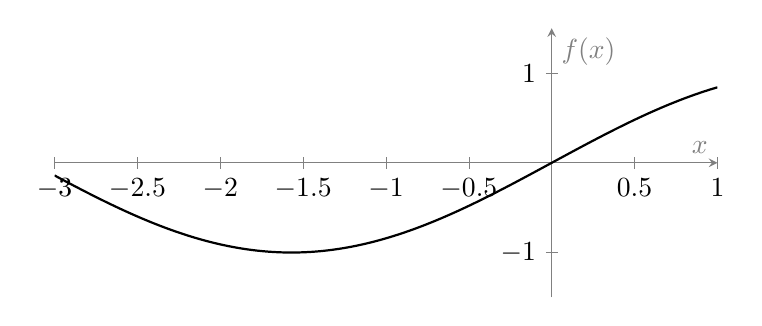
\begin{tikzpicture}
        \begin{axis}[
              width=10cm,
              height=5cm,
              axis x line=middle,
              axis y line=middle,
              xlabel={$x$},
              ylabel={$f(x)$},
              domain=-3:1,
              samples=100,
              ymin=-1.5, ymax=1.5,
              xmin=-3, xmax=1,
              legend style={at={(0.5,-0.2)},anchor=north},
              tick style={gray},
              label style={gray},
              axis line style={gray},
        ]
        % Continuous curve
        \addplot[black, thick, smooth] {sin(deg(x))};
        % Discretized points
        \end{axis}
    \end{tikzpicture}
    \caption{Continuous curve $f(x) = \sin(x)$ and its discretized version (black dots) on $[-3,1]$ with step size $h=1$.}
    \label{fig:sine}
\end{figure}


\newthought{0th Order: Match the function value.} 
We want a polynomial $P(x)$ that approximates $f(x)$ near $x_n$. Start with matching at the point itself:
\begin{equation}
    P(x_n) = f(x_n)
\end{equation}

This comes very close to what grid search does: it only looks at the function value at discrete points, without any information about how the function behaves between those points.

\begin{figure}[h]
    \centering
    % Requires: \usepackage{pgfplots}
    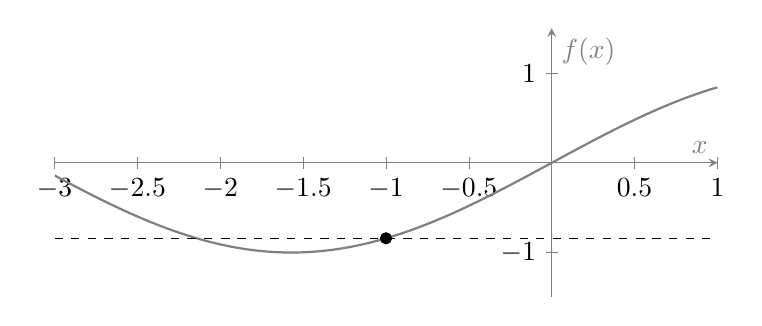
\begin{tikzpicture}
        \begin{axis}[
              width=10cm,
              height=5cm,
              axis x line=middle,
              axis y line=middle,
              xlabel={$x$},
              ylabel={$f(x)$},
              domain=-3:1,
              samples=100,
              ymin=-1.5, ymax=1.5,
              xmin=-3, xmax=1,
              legend style={at={(0.5,-0.2)},anchor=north},
              tick style={gray},
              label style={gray},
              axis line style={gray},
        ]
        % Continuous curve
        \addplot[gray, thick, smooth] {sin(deg(x))};
        % Horizontal approximation at x=-1.5
        \addplot[black, dashed, domain=-3:1] {sin(deg(-1))};
        % Mark the point at x=-1
        \addplot[black, only marks, mark=*, mark size=2pt] coordinates {(-1, {sin(deg(-1))})};
        \end{axis}
    \end{tikzpicture}
    \caption{Continuous curve $f(x) = \sin(x)$ with constant approximation $P(x) = f(-1)$ (black dashed line) anchored at $x=-1$ (black dot).}
    \label{fig:sine_constant_approx}
\end{figure}




\newthought{1st Order: Match the first derivative.}
Near $x_n$, the function's slope matters. We want $P'(x_n) = f'(x_n)$.

Adding a linear term:
\begin{equation}
    P(x) = f(x_n) + f'(x_n)(x - x_n)
\end{equation}

\begin{figure}[h]
    \centering
    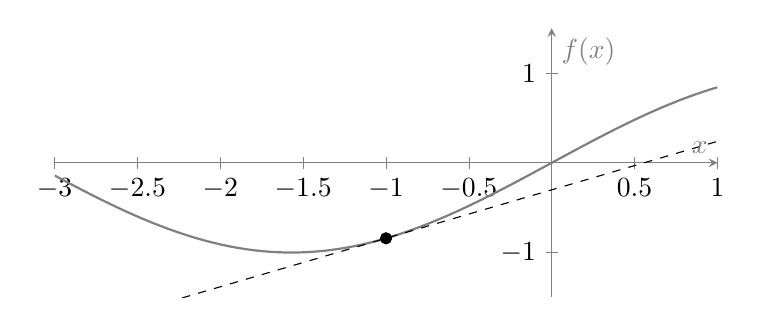
\begin{tikzpicture}
        \begin{axis}[
              width=10cm,
              height=5cm,
              axis x line=middle,
              axis y line=middle,
              xlabel={$x$},
              ylabel={$f(x)$},
              domain=-3:1,
              samples=100,
              ymin=-1.5, ymax=1.5,
              xmin=-3, xmax=1,
              legend style={at={(0.5,-0.2)},anchor=north},
              tick style={gray},
              label style={gray},
              axis line style={gray},
        ]
        % Continuous curve
        \addplot[gray, thick, smooth] {sin(deg(x))};
        % Linear approximation: tangent line at x=-1
        % f(-1) = sin(-1) ≈ -0.8414, f'(-1) = cos(-1) ≈ 0.5403
        % P(x) = sin(-1) + cos(-1)*(x - (-1)) = -0.8414 + 0.5403*(x+1)
        \addplot[black, dashed, domain=-3:1] {sin(deg(-1)) + cos(deg(-1))*(x+1)};
        % Mark the point at x=-1
        \addplot[black, only marks, mark=*, mark size=2pt] coordinates {(-1, {sin(deg(-1))})};
        \end{axis}
    \end{tikzpicture}
    \caption{Continuous curve $f(x) = \sin(x)$ with linear approximation $P(x) = f(-1) + f'(-1)(x+1)$ (black dashed tangent line) anchored at $x=-1$ (black dot).}
    \label{fig:sine_linear_approx}
\end{figure}



\newthought{2nd Order: Match the second derivative.}
The curvature captures how the slope changes. We want $P''(x_n) = f''(x_n)$.
Adding a quadratic term:
\begin{equation}
    P(x) = f(x_n) + f'(x_n)(x - x_n) + \frac{f''(x_n)}{2}(x - x_n)^2
\end{equation}


\begin{figure}[h]
    \centering
    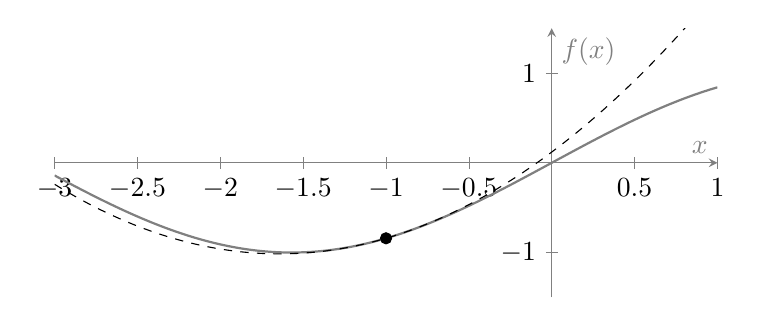
\begin{tikzpicture}
        \begin{axis}[
              width=10cm,
              height=5cm,
              axis x line=middle,
              axis y line=middle,
              xlabel={$x$},
              ylabel={$f(x)$},
              domain=-3:1,
              samples=100,
              ymin=-1.5, ymax=1.5,
              xmin=-3, xmax=1,
              legend style={at={(0.5,-0.2)},anchor=north},
              tick style={gray},
              label style={gray},
              axis line style={gray},
        ]
        % Continuous curve
        \addplot[gray, thick, smooth] {sin(deg(x))};
        % Quadratic approximation: Taylor expansion at x=-1
        % f(-1) = sin(-1) ≈ -0.8414, f'(-1) = cos(-1) ≈ 0.5403, f''(-1) = -sin(-1) ≈ 0.8414
        % P(x) = sin(-1) + cos(-1)*(x+1) + (-sin(-1))/2*(x+1)^2
        \addplot[black, dashed, domain=-3:1] {sin(deg(-1)) + cos(deg(-1))*(x+1) + (-sin(deg(-1)))/2*(x+1)^2};
        % Mark the point at x=-1
        \addplot[black, only marks, mark=*, mark size=2pt] coordinates {(-1, {sin(deg(-1))})};
        \end{axis}
    \end{tikzpicture}
    \caption{Continuous curve $f(x) = \sin(x)$ with quadratic approximation $P(x) = f(-1) + f'(-1)(x+1) + \frac{f''(-1)}{2}(x+1)^2$ (black dashed parabola) anchored at $x=-1$ (black dot).}
    \label{fig:sine_quadratic_approx}
\end{figure}



\marginnote{\newthought{Why divide by 2?} When we differentiate $(x-x_n)^2$ twice, we get 2. 
So if we want $P''(x_n) = f''(x_n)$, we need to divide by 2 to cancel this factor.}




\newthought{nth Order: General pattern.}

\newthought{The Taylor expansion} of a function $f$ around a point $x_n$ is given by:
\begin{equation*}
    f(x) = f(x_n) + f'(x_n)(x - x_n) + \frac{f''(x_n)}{2!}(x - x_n)^2 + \frac{f'''(x_n)}{3!}(x - x_n)^3 + \cdots
\end{equation*}

Or more compactly:
\begin{equation}
    f(x) = \sum_{k=0}^{\infty} \frac{f^{(k)}(x_n)}{k!}(x - x_n)^k
\end{equation}



\marginnote{\newthought{Around a point.} Visually we can see that the approximations are anchored on a specific point $x_n$. 
The Taylor expansion is a local approximation.}



\newthought{Why linear is enough for Newton?} \\
We want to solve $f(x^*) = 0$, not compute $f(x)$ as best as we can.
Improving an approximation of course comes with a cost: We need to compute higher derivatives 
and evaluate more complex polynomials.
In numerical computations we always need to decide where to cut off the Taylor series. 
We do so at some finite order, and the linear term is the first non-constant term that 
gives us directional information.

\index{quadratic convergence}

\newthought{Deriving the convergence rate}. Recall from Chapter 3, that a method is convergent if our approximation reaches a specific stable limit. 
For Newton's method finding a root $x^*$ where $f(x^*) = 0$, we want:
\begin{equation}
    |x_n - x^*| \to 0 \quad \text{as } n \to \infty
\end{equation}

Thanks to the Taylor expansion, we can quantify how fast the error decreases.\\

Let $e_n = x_n - x^*$ be the error at iteration $n$. 
Applying a 2nd Order Taylor expansion to $f$ around the true root $x^*$:
\begin{equation}
    f(x_n) = f(x^*) + f'(x^*)(x_n - x^*) + \frac{f''(\xi)}{2}(x_n - x^*)^2,
\end{equation}

where $\xi$ is some point between $x_n$ and $x^*$. Since $f(x^*) = 0$, this simplifies to:
\begin{equation}
    f(x_n) = f'(x^*) \cdot e_n + \frac{f''(\xi)}{2} e_n^2
\end{equation}
Where $e_n = x_n - x^*$ is the error at iteration $n$.

\newthought{Now apply Newton's formula:}
\begin{align*}
    e_{n+1} &= x_{n+1} - x^* \\
    &= x_n - \frac{f(x_n)}{f'(x_n)} - x^* \\
    &= (x_n - x^*) - \frac{f(x_n)}{f'(x_n)} \\
    &= e_n - \frac{f(x_n)}{f'(x_n)}
\end{align*}

and substitute the simplified Taylor expansion for $f(x_n)$:
\begin{equation}
    e_{n+1} = e_n - \frac{f'(x^*) \cdot e_n + \frac{f''(\xi)}{2} e_n^2}{f'(x_n)}.
\end{equation}

\newthought{For points close to $x^*$,}  we can make the assumption that $f'(x_n) \approx f'(x^*)$,

\marginnote{\newthought{Notice the assumption play out:} $10^{-1} \to 10^{-2} \to 10^{-3} \to 10^{-6} \to 10^{-12}$.
Once we're close enough and our assumptions hold (after iteration 2), the error squares perfectly, demonstrating quadratic convergence.}


\begin{equation}
    e_{n+1} \approx e_n - \frac{f'(x^*) \cdot e_n + \frac{f''(\xi)}{2} e_n^2}{f'(x^*)} = e_n - e_n - \frac{f''(\xi)}{2f'(x^*)} e_n^2
\end{equation}

which makes the first order error term cancel out, leaving us with:

\begin{equation}
    e_{n+1} \approx -\frac{f''(\xi)}{2f'(x^*)} e_n^2
\end{equation}

\newthought{In more abstract terms,} we can write this as:
\begin{equation}
    |e_{n+1}| \leq C \cdot |e_n|^2
\end{equation}
Which means that the error at the next iteration is approximately proportional to the square of the current error, where $C$ is a constant that depends on the function's curvature and slope at the root.

\newthought{This is quadratic convergence.} 

\vspace{1.5em}
Let's come back to our introductory example of computing $\sqrt{2}$ with Newton starting from $x_0 = 2$:

\begin{table*}[h]
\centering
\begin{tabular}{p{0.25\textwidth}p{0.37\textwidth}p{0.38\textwidth}}
\toprule
\textbf{$n$} & \textbf{$x_n$} & \textbf{$|e_n|$ (error)} \\
\midrule
0 & 2.000000000 & $5.86 \times 10^{-1}$ \\
1 & 1.500000000 & $8.58 \times 10^{-2}$ \\
2 & 1.416666667 & $2.45 \times 10^{-3}$ \\
3 & 1.414215686 & $2.13 \times 10^{-6}$ \\
4 & 1.414213562 & $4.5 \times 10^{-12}$ \\
\bottomrule
\end{tabular}
\vspace{2em}
\caption{Newton's method for computing $\sqrt{2}$. See how the error approximately squares each iteration.}
\label{tab:newton_sqrt2}
\end{table*}



\index{Newton failure modes}
\newthought{Newton's method can fail} in several ways, which we will endure for now, 
and for which we will find solutions later on. As a brain teaser, it is a nice exercise to 
visualize the failure modes in this plot: 

\begin{figure}[h]
    \centering
    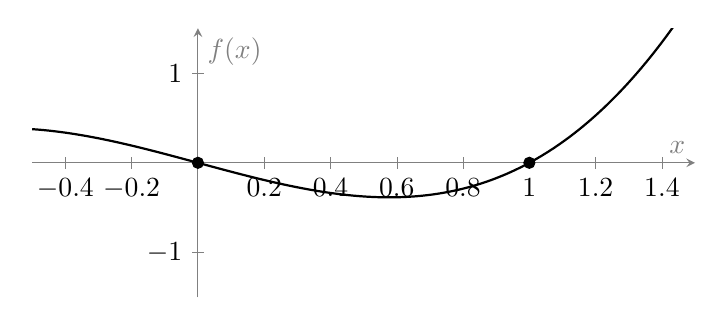
\begin{tikzpicture}
        \begin{axis}[
            width=10cm,
            height=5cm,
            axis x line=middle,
            axis y line=middle,
            xlabel={$x$},
            ylabel={$f(x)$},
            domain=-0.5:1.5,
            samples=100,
            ymin=-1.5, ymax=1.5,
            xmin=-0.5, xmax=1.5,
            tick style={gray},
            label style={gray},
            axis line style={gray},
        ]
        % f(x) = x^3 - x (has roots at -1, 0, 1)
        \addplot[black, thick, smooth] {x^3 - x};
        % Mark the roots (only 0 and 1 are in the visible range)
        \addplot[black, only marks, mark=*, mark size=2pt] coordinates {(0, 0) (1, 0)};
        \end{axis}
    \end{tikzpicture}
    \caption{$f(x) = x^3 - x$ has multiple roots. Newton's method can fail in several ways: 
    zero derivative (if $f'(x_n) = 0$, the tangent is horizontal and doesn't cross the axis), 
    oscillation (especially for symmetrical functions Newton can cycle between points), 
    and ambiguous starting point selection ($x_0$, heavily influences which root is found).}
    \label{fig:newton_multiple_roots}
\end{figure}






\vspace{1em}

\index{Secant method}

\newthought{Now something we can not endure}, is if we can't compute $f'(x)$.\\

\marginnote{\newthought{This can happen because:} 
\begin{itemize}
    \item The derivative is expensive to compute.
    \item The function is given as a black box (e.g., a simulation).
    \item The function isn't differentiable everywhere.
\end{itemize}}

\marginnote{\newthought{In deep learning,} we painstakingly make sure to design our loss functions, 
and activation functions to be differentiable, so that we we make sure that our gradients flow.}

\section{Secant Method}
Here comes a clever way to approximate the 
derivative using only function evaluations, eliminating the need for an explicit derivative.

\vspace{2em}
\newthought{A poor man's derivative.} Approximate the derivative using two recent points:
\begin{equation*}
    f'(x_n) \approx \frac{f(x_n) - f(x_{n-1})}{x_n - x_{n-1}}
\end{equation*}

\vspace{2em}
Visually this is the slope of the secant line connecting the points $(x_{n-1}, f(x_{n-1}))$ and $(x_n, f(x_n))$ on the graph of $f$:
\vspace{2em}
\begin{figure}[h]
    \centering
    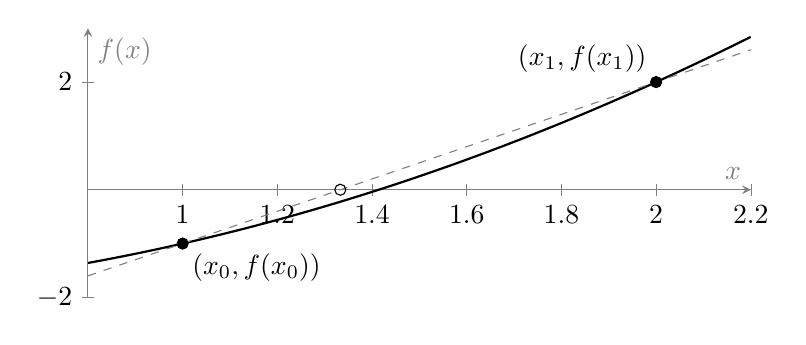
\begin{tikzpicture}
        \begin{axis}[
            width=10cm,
            height=5cm,
            axis x line=middle,
            axis y line=middle,
            xlabel={$x$},
            ylabel={$f(x)$},
            domain=0.8:2.2,
            samples=100,
            ymin=-2, ymax=3,
            xmin=0.8, xmax=2.2,
            tick style={gray},
            label style={gray},
            axis line style={gray},
        ]
        % The function f(x) = x^2 - 2
        \addplot[black, thick, smooth] {x^2 - 2};

        % Secant line through (1, -1) and (2, 2)
        \addplot[gray, dashed, domain=0.8:2.2] {3*x - 4};
        % Points
        \addplot[black, only marks, mark=*, mark size=2pt] coordinates {(1, -1) (2, 2)};
        \node[below right] at (axis cs:1,-1) {$(x_0, f(x_0))$};
        \node[above left] at (axis cs:2,2) {$(x_1, f(x_1))$};

        % Secant crosses at x = 4/3
        \addplot[black, only marks, mark=o, mark size=2pt] coordinates {(1.333, 0)};

        \end{axis}
    \end{tikzpicture}
    \caption{Secant method: the line through $(x_0, f(x_0))$ and $(x_1, f(x_1))$ gives the next approximation $x_2$.}
    \label{fig:secant_method}
\end{figure}

\vspace{2em}
\newthought{Note,} that this also means that we need two initial guesses $x_0$ and $x_1$ to start the iteration,
instead of just one for Newton's method.

Substituting into Newton's formula, gives us the iterative Secant method:
\begin{equation}
    x_{n+1} = x_n - f(x_n) \cdot \frac{x_n - x_{n-1}}{f(x_n) - f(x_{n-1})}
\end{equation}

\vspace{2em}
\newthought{And here's the algorithmic version formulated as a loop:}

\begin{algorithm}[H]
\caption{Secant Method}
\begin{algorithmic}[1]
    \Require Initial guesses $x_0$, $x_1$, function $f$, tolerance $\varepsilon$
    \While{$|f(x_1)| > \varepsilon$}
        \State Compute secant slope: $s \gets (f(x_1) - f(x_0)) / (x_1 - x_0)$
        \State Store previous: $x_{\text{old}} \gets x_1$
        \State Update: $x_1 \gets x_1 - f(x_1) / s$
        \State $x_0 \gets x_{\text{old}}$
    \EndWhile
    \Return $x_1$
\end{algorithmic}
\end{algorithm}




















% ==============================================================================================
% STUDENT ACTIVATION BLOCK

\newpage
\section{Examples \& Exercises}


\begin{figure}[h]
    \centering
    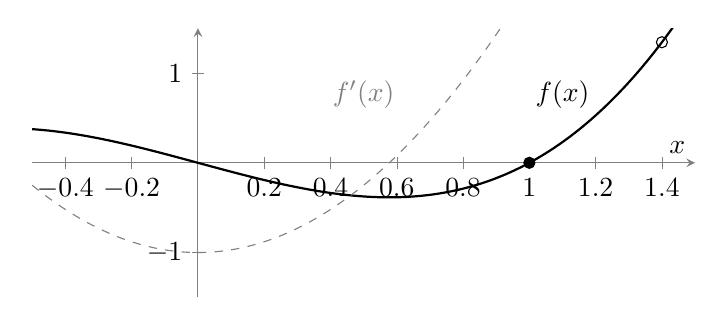
\begin{tikzpicture}
        \begin{axis}[
            width=10cm,
            height=5cm,
            axis x line=middle,
            axis y line=middle,
            xlabel={$x$},
            domain=-0.5:1.5,
            samples=100,
            ymin=-1.5, ymax=1.5,
            xmin=-0.5, xmax=1.5,
            tick style={gray},
            label style={black},
            axis line style={gray},
        ]
        % f(x) = x^3 - x (has roots at -1, 0, 1)
        \addplot[black, thick, smooth] {x^3 - x};
        % label for the function
        \node[above, black] at (axis cs:1.1,0.5) {$f(x)$};
        % Derivative f'(x) = 3x^2 - 1
        \addplot[gray, dashed, smooth] {3*x^2 - 1};
        % label for the derivative
        \node[above, gray] at (axis cs:0.5,0.5) {$f'(x)$};
        % Mark the roots (only 0 and 1 are in the visible range)
        \addplot[black, only marks, mark=*, mark size=2pt] coordinates {(1, 0)};
        % add a o mark at x=1.4 on the curve for x_0
        \addplot[black, only marks, mark=o, mark size=2pt] coordinates {(1.4, {1.4^3 - 1.4})};
        \end{axis}
    \end{tikzpicture}
    \caption{$f(x) = x^3 - x$ has multiple roots. We assume the root at $x = 1$ is the target. The gray dashed line shows the derivative $f'(x) = 3x^2 - 1$.}
    \label{fig:newton_excercises}
\end{figure}

\marginnote{\newthought{Code} can be found at \url{https://github.com/Quillstacks/lecturecode_numericalmethods.git}.}

\newthought{Newton by hand.} Find the root of $f(x) = x^3 - x = 0$ solving Newton's method geometrically, and then by hand.
The roots are at $x = -1, 0, 1$. Let's find the root at $x = 1$ starting from $x_0 = 1.4$. The 1st order Taylor expansion around $x_n$ gives us:
\begin{align*}
    f(x) \approx f(x_n) + f'(x_n)(x - x_n),\\
    f(x_n) \approx f(x) - f'(x_n)(x - x_n)
\end{align*}

We have $f(x) = x^3 - x = 0$, with  $f'(x) = 3x^2 - 1$, so we can rearrange to find the next guess,
starting from $x_0 = 1.4$:
\begin{align*}
    x_1 &= x_0 - \frac{f(x_0)}{f'(x_0)} \\
    &= x_0 - \frac{x_0^3 - x_0}{3x_0^2 - 1} \\
    &= 1.4 - \frac{2.744 - 1.4}{5.88 - 1} \\
    &= 1.4 - \frac{1.344}{4.88} \approx 1.127 \\
    x_2 &= 1.127 - \frac{1.127^3 - 1.127}{3(1.127)^2 - 1} \\
    &\approx 1.127 - \frac{0.432}{2.808} \\
    &\approx 0.976 \\
    x_3 &= 0.976 - \frac{0.976^3 - 0.976}{3(0.976)^2 - 1} \\
    &\approx 0.976 - \frac{-0.072}{1.857} \\
    &\approx 1.014
\end{align*}

The root at $x = 1$ is found quickly.


\newthought{Secant by hand.} Apply the Secant method to the same problem with $x_0 = 1.2$, $x_1 = 1.4$.
Again first geometrically, then by hand.

\begin{align*}
    x_2 &= x_1 - f(x_1) \cdot \frac{x_1 - x_0}{f(x_1) - f(x_0)} \\
    &= 1.4 - (0.744) \cdot \frac{1.4-1.2}{0.744 - 0.128} \\
    &= 1.4 - 0.744 \cdot \frac{0.2}{0.616} \\
    &\approx 1.4 - 0.241 \\
    &\approx 1.159 \\
    x_3 &= 1.159 - f(1.159) \cdot \frac{1.159 - 1.4}{f(1.159) - f(1.4)} \\
     &\approx 1.159 - (0.283) \cdot \frac{-0.241}{0.283 - 0.744} \\
     &\approx 1.159 - 0.283 \cdot \frac{-0.241}{-0.461} \\
     &\approx 1.159 - 0.283 \cdot 0.522 \\
     &\approx 1.159 - 0.148 \\
     &\approx 1.011
\end{align*}


\vspace{2em}
\newthought{Geometrical Failure Search.} 
Find starting points $x_0$ for different failure modes: One where Newton's method fails due to zero derivative, 
one where it converges to a non-target root, and one where it oscillates between points.


\newthought{Enter the machine.} Let's have a look on the convergence and convergence rates 
of Grid-Search, Newton and Secant method in Python. 
Then continue to experiment with differentstarting points, and observe the 
failure modes in practice. Try to first find the starting points geometrically, 
then try finding them analytically, 
before finally moving over to verifying in code.




\section{Self-Reflection and Recap}

\newthought{Self-Reflection} Questions to guide your understanding:
\begin{itemize}
    \item What is the main advantage of using Newton's method over Grid-Search?
    \item Why is a linear approximation sufficient for finding roots? What does the Taylor expansion tell us about this choice?
    \item Why is quadratic convergence so powerful? How many iterations would Newton need to go from error $10^{-1}$ to error $10^{-16}$?
    \item In what situations would you prefer Secant over Newton? Why not in others?
\end{itemize}

\newthought{Recap} of Key Concepts:
\begin{itemize}
    \item Newton-Raphson gives (limited) convergence guarantees near simple roots.
    \item Taylor expansion provides a systematic way to approximate functions locally.
    \item You saw how Taylor expansion justifies the linear approximation in Newton's method and explains its quadratic convergence and allows to estimate the error in each iteration.
    \item In situations where the derivative is difficult to compute, the Secant method approximates the derivative from two points and converges.
\end{itemize}


\marginnote{\newthought{Teaser.} How can we make sure that we find the global solution, and not just a local one?}

\newthought{Local methods find local solutions.} Newton converges to whatever optimum is nearby, 
it is also prone to oscillate between points, or diverge if the derivative is zero or near zero. In the next chapter, we will reformulate the root finding into an optimization problem.
And from there we'll explore how to go on and handle global optimization when the landscape has many valleys or is otherwise pathologically difficult.



%%%%%%%%%%%%%%%%%%%%%%%%%%%%%%%%%%%%%%%%%%%%%%%%%%%%%%%%%%%%%%%%%%%%%%%%%%%%%%

\input{chapters/5_global_optimization.tex}
\index{numerical integration}
\index{stochastic gradient descent}
\chapter{Numerical Integration}
\printchapterversion{6_integration_and_sgd}
\newthought{Smooth Operator.}


% ==============================================================================================
% INTRODUCTION BLOCK

\section{The Why}
\index{numerical integration!motivation}

\marginnote{\newthought{Melts all your memories} \href{https://open.spotify.com/track/1Hv1VTm8zeOeybub15mA2R?si=2b063718fca34b6a}{ and change into gold}}

\newthought{In the previous chapter,} we explored global optimization strategies to escape local minima.
Imagine you are optimizing a function with thousands of tiny, sharp local minima like a high-frequency version of Shekel’s Foxholes. 
A gradient descent algorithm will get stuck instantly in the first microscopic pothole it finds.


\newthought{The solution for this} is one that will feel familiar, but probably did go unnoticed until now: Numerical integration. 
\begin{equation}
    I = \int_a^b f(x) \, dx
\end{equation}

\newthought{This gives us good reasons} to understand numerical integration,
\begin{itemize}
    \item as it allows us to smoothen the loss landscape and make optimization methods more robust.
    \item as it tends to find more robust optima due to the averaging effect\cite{batchtraining} of a region.
\end{itemize}


\newthought{In deep learning} stochastic gradient descent (SGD) is the workhorse optimization algorithm.

\marginnote{\newthought{Monte Carlo} is a strategy which basically solves problems by random sampling. Embrace the beauty: }

It is a Monte Carlo\cite{randomsearch}\cite{montecarlodropout} method that estimates the gradient of the loss function by averaging over the gradient of a 
random mini-batch of data points. We are lucky to have numerical integration around, as it would be prohibitive expensive to train models on large-scale datasets.









\newpage
\subsection{Hands On Experience}
\index{numerical integration!hands-on}
\index{discretization} \index{approximation} \index{stepsize} \index{interval}

We already know how to discretize a continuous function, and how to handle finite precision and systems with sparse information at discrete points.


\begin{figure}[h]
    \centering
    % Requires: \usepackage{pgfplots}
    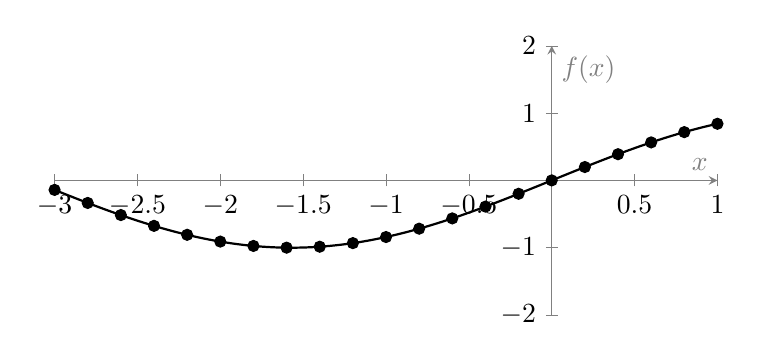
\begin{tikzpicture}
        \begin{axis}[
              width=10cm,
              height=5cm,
              axis x line=middle,
              axis y line=middle,
              xlabel={$x$},
              ylabel={$f(x)$},
              domain=-3:1,
              samples=100,
              ymin=-2, ymax=2,
              xmin=-3, xmax=1,
              legend style={at={(0.5,-0.2)},anchor=north},
              tick style={gray},
              label style={gray},
              axis line style={gray},
        ]
        % Continuous curve
        \addplot[black, thick, smooth] {sin(deg(x))};
        % Discretized points every 0.2 from -3 to 1
        \addplot[black, only marks, mark=*] coordinates {
            (-3.0, -0.1411)
            (-2.8, -0.33499)
            (-2.6, -0.51504)
            (-2.4, -0.67546)
            (-2.2, -0.80850)
            (-2.0, -0.90930)
            (-1.8, -0.97385)
            (-1.6, -0.99957)
            (-1.4, -0.98545)
            (-1.2, -0.93204)
            (-1.0, -0.84147)
            (-0.8, -0.71736)
            (-0.6, -0.56464)
            (-0.4, -0.38942)
            (-0.2, -0.19867)
            (0.0, 0.0)
            (0.2, 0.19867)
            (0.4, 0.38942)
            (0.6, 0.56464)
            (0.8, 0.71736)
            (1.0, 0.84147)
        };
        \end{axis}
    \end{tikzpicture}
    \caption{Continuous curve $f(x) = \sin(x)$ and its discretized version (black dots) on $[-3,1]$ with step size $h=0.2$.}
    \label{fig:discretizationlowfrequency}
\end{figure}

\newthought{The Shekel function}, as a high-frequency function, did pose a challenge for global optimization, yet did not render our general approaches obsolete. We still discretize and treat these functions as we are used to.

\begin{figure}[h]
    \centering
    % Requires: \usepackage{pgfplots}
    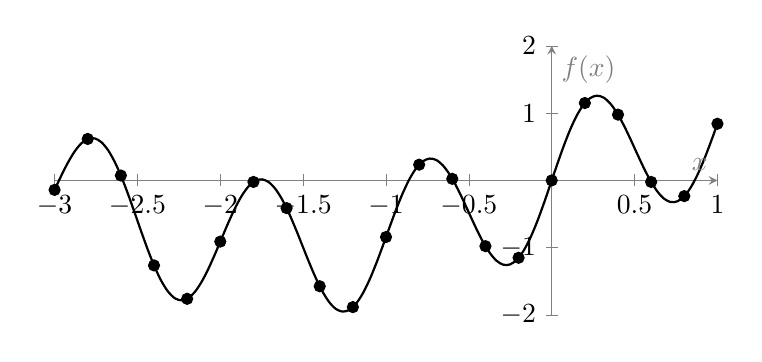
\begin{tikzpicture}
        \begin{axis}[
              width=10cm,
              height=5cm,
              axis x line=middle,
              axis y line=middle,
              xlabel={$x$},
              ylabel={$f(x)$},
              domain=-3:1,
              samples=100,
              ymin=-2, ymax=2,
              xmin=-3, xmax=1,
              legend style={at={(0.5,-0.2)},anchor=north},
              tick style={gray},
              label style={gray},
              axis line style={gray},
        ]
        % Continuous curve: sum of sin(x) and sin(2πx)
        \addplot[black, thick, smooth] {sin(deg(x)) + sin(360*x)};
        % Discretized points every 0.2 from -3 to 1 for f(x)=sin(x)+sin(2\pi x)
        \addplot[black, only marks, mark=*] coordinates {
            (-3.0, -0.14112)
            (-2.8, 0.61607)
            (-2.6, 0.07275)
            (-2.4, -1.26325)
            (-2.2, -1.75955)
            (-2.0, -0.90930)
            (-1.8, -0.02279)
            (-1.6, -0.41179)
            (-1.4, -1.57323)
            (-1.2, -1.88310)
            (-1.0, -0.84147)
            (-0.8, 0.23370)
            (-0.6, 0.02314)
            (-0.4, -0.97720)
            (-0.2, -1.14973)
            (0.0, 0.0)
            (0.2, 1.14973)
            (0.4, 0.97720)
            (0.6, -0.02314)
            (0.8, -0.23370)
            (1.0, 0.84147)
        };
        \end{axis}
    \end{tikzpicture}
    \caption{Continuous curve $f(x)=\sin(x)+\sin(2\pi x)$ and its discretized version (black dots) on $[-3,1]$ with step size $h=0.2$.}
    \label{fig:discretizationhighfrequency}
\end{figure}

\newthought{Taking a closer look at any} local minima shows how the high-frequency loss landscape will nudge our optimization algorithm into the nearest local minimum.
For example at $x=0.6$ or $x=-0.4$.

\begin{figure}[h]
    \centering
    % Requires: \usepackage{pgfplots}
    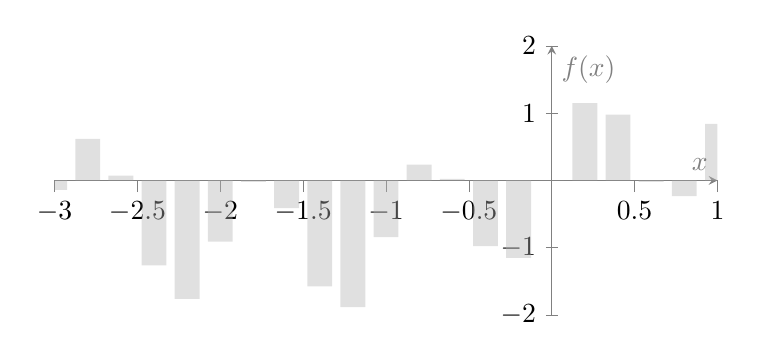
\begin{tikzpicture}
        \begin{axis}[
              width=10cm,
              height=5cm,
              axis x line=middle,
              axis y line=middle,
              xlabel={$x$},
              ylabel={$f(x)$},
              domain=-3:1,
              samples=100,
              ymin=-2, ymax=2,
              xmin=-3, xmax=1,
              legend style={at={(0.5,-0.2)},anchor=north},
              tick style={gray},
              label style={gray},
              axis line style={gray},
              ybar,
              bar width=0.15,
        ]
        % Bar plot for discretized summed values (h=0.2)
        \addplot[fill=gray!60, fill opacity=0.4, draw=none] coordinates {
            (-3.0, -0.14112)
            (-2.8, 0.61607)
            (-2.6, 0.07275)
            (-2.4, -1.26325)
            (-2.2, -1.75955)
            (-2.0, -0.90930)
            (-1.8, -0.02279)
            (-1.6, -0.41179)
            (-1.4, -1.57323)
            (-1.2, -1.88310)
            (-1.0, -0.84147)
            (-0.8, 0.23370)
            (-0.6, 0.02314)
            (-0.4, -0.97720)
            (-0.2, -1.14973)
            (0.0, 0.0)
            (0.2, 1.14973)
            (0.4, 0.97720)
            (0.6, -0.02314)
            (0.8, -0.23370)
            (1.0, 0.84147)
        };
        \end{axis}
    \end{tikzpicture}
    \caption{Continuous curve $f(x)=\sin(x)+\sin(2\pi x)$ and its discretized version (black dots) on $[-3,1]$ with step size $h=0.2$.}
    \label{fig:discretizationhighfrequency}
\end{figure}



\newthought{Consider approximation by numerical integration.} Let's see what it does at $x=-0.4$, instead of 
solving directly for: 

\begin{equation}
    f(-0.4) = -0.97720,
\end{equation}

let's approximate the value through integration with width \\ $h=0.2$:

\begin{align*}
    h \cdot f(-0.4) &\approx \int_{-0.5}^{-0.3} f(x) \, dx \\ 
            &\approx \frac{h}{2}[f(-0.5) + f(-0.3)] \\
            &\approx 0.2 \cdot \frac{-1.14973 - 0.97720}{2} \\
            &= -0.11285
\end{align*}
\begin{align*}
    f(-0.4) &\approx \frac{-1.14973 - 0.97720}{2} \\
            &= -1.06347
\end{align*}

\newthought{This is a much better approximation} having global optima in mind, than the direct evaluation at $x=-0.4$ which gave us $-0.97720$.
The numerical integration gave us a correction of the local loss landscape towards higher losses at this local minima.
The next figure shows the effect of this smoothing on the whole curve.

\begin{figure}[h]
    \centering
    % Requires: \usepackage{pgfplots}
    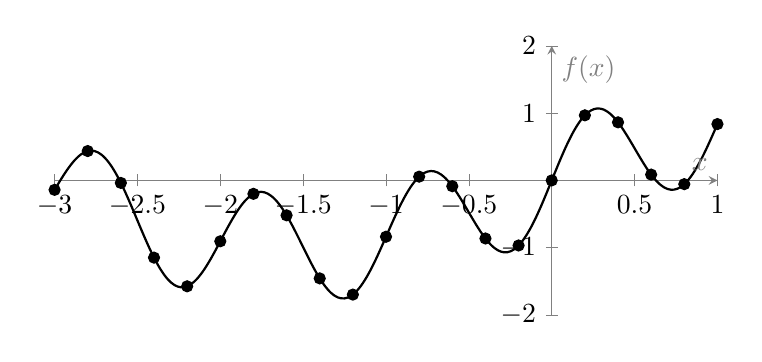
\begin{tikzpicture}
        \begin{axis}[
              width=10cm,
              height=5cm,
              axis x line=middle,
              axis y line=middle,
              xlabel={$x$},
              ylabel={$f(x)$},
              domain=-3:1,
              samples=100,
              ymin=-2, ymax=2,
              xmin=-3, xmax=1,
              legend style={at={(0.5,-0.2)},anchor=north},
              tick style={gray},
              label style={gray},
              axis line style={gray},
        ]
        % Smoothed continuous curve: average of neighbours at ±h/2 (h=0.2 → ±0.1)
        \addplot[black, thick, smooth, domain=-3:1, samples=200] {((sin(deg(x-0.1)) + sin(360*(x-0.1)) + sin(deg(x+0.1)) + sin(360*(x+0.1)))/2)};
        % Smoothed discretized points every 0.2 from -3 to 1 using the same neighbour-average
        \addplot[black, only marks, mark=* , samples at={-3.0,-2.8,-2.6,-2.4,-2.2,-2.0,-1.8,-1.6,-1.4,-1.2,-1.0,-0.8,-0.6,-0.4,-0.2,0.0,0.2,0.4,0.6,0.8,1.0}] {((sin(deg(x-0.1)) + sin(360*(x-0.1)) + sin(deg(x+0.1)) + sin(360*(x+0.1)))/2)};
        \end{axis}
    \end{tikzpicture}
    \caption{Continuous curve $f(x)=\sin(x)+\sin(2\pi x)$ and its discretized version (black dots) on $[-3,1]$ with step size $h=0.2$, and smoothed by numerical integration with interval length $h$.}
    \label{fig:discretizationhighfrequencysmoothed}
\end{figure}

\newthought{The smoothing} becomes even more apparent when integrating over larger intervals in general, or in our engineered example when choosing $h$ such that the frequency of the noisy signal gets averaged out.

\marginnote{\newthought{What if,} we would be integrating over an interval which results in destructive inference of the underlying higher frequency sine curve? Think wavelengths.}

\begin{figure}[h]
    \centering
    % Requires: \usepackage{pgfplots}
    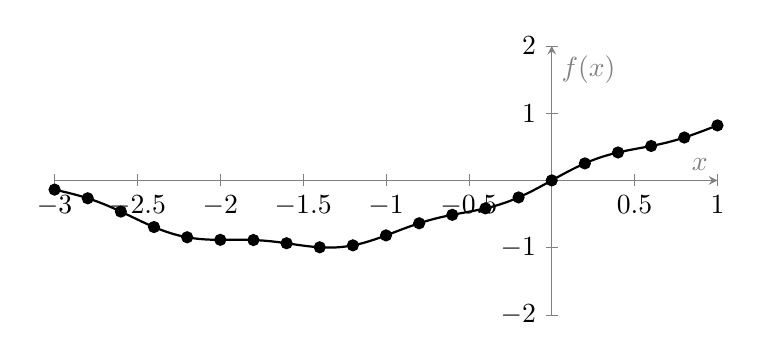
\begin{tikzpicture}
        \begin{axis}[
              width=10cm,
              height=5cm,
              axis x line=middle,
              axis y line=middle,
              xlabel={$x$},
              ylabel={$f(x)$},
              domain=-3:1,
              samples=100,
              ymin=-2, ymax=2,
              xmin=-3, xmax=1,
              legend style={at={(0.5,-0.2)},anchor=north},
              tick style={gray},
              label style={gray},
              axis line style={gray},
        ]
        % Smoothed continuous curve: average of neighbours at ±h/2 (choose h=0.48 → ±0.24 to get close to cancel sin(2\pi x))
        \addplot[black, thick, smooth, domain=-3:1, samples=200] {((sin(deg(x-0.24)) + sin(360*(x-0.24)) + sin(deg(x+0.24)) + sin(360*(x+0.24)))/2)};
        % Smoothed discretized points every 0.2 from -3 to 1 using the same neighbour-average
        \addplot[black, only marks, mark=* , samples at={-3.0,-2.8,-2.6,-2.4,-2.2,-2.0,-1.8,-1.6,-1.4,-1.2,-1.0,-0.8,-0.6,-0.4,-0.2,0.0,0.2,0.4,0.6,0.8,1.0}] {((sin(deg(x-0.24)) + sin(360*(x-0.24)) + sin(deg(x+0.24)) + sin(360*(x+0.24)))/2)};
        \end{axis}
    \end{tikzpicture}
    \caption{Continuous curve $f(x)=\sin(x)+\sin(2\pi x)$ and its discretized version (black dots) on $[-3,1]$ with step size $h=0.2$, smoothed by neighbour averaging with $h=0.48$ (so $h/2=0.24$ gets close to cancel the $\sin(2\pi x)$ component).}
    \label{fig:discretizationhighfrequencysmoothedOne}
\end{figure}

\newthought{While you have} seen the smoothing effect driven by the interval size, the approximation of the interval so far is a pretty coarse approximation, relying on two points only.

\vspace{2.5em}
\newthought{The Learning Objectives} of this chapter will provide you with the abilities to:
\begin{itemize}
    \item Derive and apply the midpoint method, trapezoid and Simpson's rules for numerical integration
    \item Understand composite rules for improved accuracy
    \item Know about Lagrange interpolation and how it relates to quadrature rules
    \item Understand how the curse of dimensionality motivates Monte Carlo 
    \item Derive and apply Monte Carlo integration for high-dimensional problems
    \item Apply Monte Carlo integration and recognize that batch averaging in ML is numerical integration
\end{itemize}








% ==============================================================================================
% MAIN THEORY BLOCK

\newpage
\subsection{Methods of Numerical Intgration}
\vspace{1em}

\newthought{The most trivial approximation of integrals} is using a single discretized value. 


\begin{align*}
    I &= \int_a^b f(x)\, dx. \\ 
    I &= \frac{b-a}{n} \cdot f\left(\frac{a+b}{2}\right) \\
    I &= h \cdot f(m)
\end{align*}

It is easy to see that the height of the rectangle is the value at the midpoint, and the width is $h$.

We can further refine the approximation of the integral by dividing $[a, b]$ into $n$ subintervals of equal width $h$, and summing the contributions from each interval.
This is also known as Riemann sum approximation, and can be expressed as:
\begin{align*}
    \int_a^b f(x)\, dx &\approx \sum_{i=0}^{n-1} \int_{x_i}^{x_{i+1}} f(x)\, dx \\
    &\approx \sum_{i=0}^{n-1} h \cdot f(m_i) \\
\end{align*}
where $x_i = a + i h$ for $i = 0, 1, \ldots, n$.

\marginnote{\newthought{On the interval $[a, b]$}, the midpoint value is $f(m)$. With left endpoint, the height is $f(a)$; with right endpoint, the height is $f(b)$.}

\newthought{The midpoint rule} of these composite intervals uses the midpoint, which is the average of the endpoints, of each interval, 
which often gives better results than left or right endpoint methods. Intuitively, this is because the midpoint approximates the curvature of the function better on the interval.

\begin{figure}[h]
    \centering
    % Requires: \usepackage{pgfplots}
    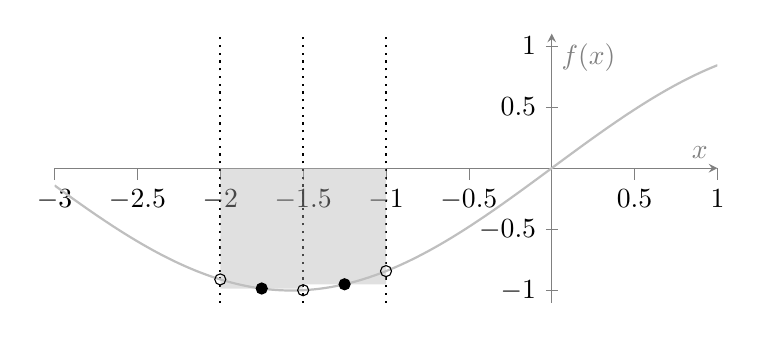
\begin{tikzpicture}
        \begin{axis}[
              width=10cm,
              height=5cm,
              axis x line=middle,
              axis y line=middle,
              xlabel={$x$},
              ylabel={$f(x)$},
              domain=-3:1,
              samples=100,
              ymin=-1.1, ymax=1.1,
              xmin=-3, xmax=1,
              legend style={at={(0.5,-0.2)},anchor=north},
              tick style={gray},
              label style={gray},
              axis line style={gray},
              ybar,
              bar width=0.5,
        ]
                % Vertical dotted guide lines (use axis coordinates to avoid interfering with plots)
                    \draw[dotted, thick, black] (axis cs:-2,-1.1) -- (axis cs:-2,1.1);
                    \draw[dotted, thick, black] (axis cs:-1.5,-1.1) -- (axis cs:-1.5,1.1);
                    \draw[dotted, thick, black] (axis cs:-1,-1.1) -- (axis cs:-1,1.1);
        % Gray bars for midpoint rule intervals (no gap)
        \addplot[fill=gray!60, fill opacity=0.4, draw=none] coordinates {
            (-1.75, -0.98363)
            (-1.25, -0.94898)
        };
        % Continuous curve: sin(x) in light gray
        \addplot[gray!50, thick, smooth] {sin(deg(x))};
        % Discretized points at midpoints
        \addplot[black, only marks, mark=*] coordinates {
            (-1.75, -0.98363)
            (-1.25, -0.94898)
        };
        % Discretized points at endpoints
        \addplot[black, only marks, mark=o] coordinates {
            (-2, -0.90930)
            (-1.5, -0.99749)
            (-1, -0.84147)
        };
        \end{axis}
    \end{tikzpicture}
    \caption{Continuous curve $f(x)=\sin(x)$ and midpoint rule integrals (gray bars) for $a=-2$, $b=-1$, $h=0.5$. Black dots: midpoints. Circles: endpoints.
    The bars now touch, illustrating the midpoint rule without a gap.}
    \label{fig:midpointrule}
\end{figure}


\newthought{Increasing the number of subintervals} reduces the error.
\marginnote{\newthought{Doubling the sub intervals} reduced error by $\sim 4\times$. This suggests $O(h^2)$ convergence.}
This of course comes at the cost of more function evaluations, and thus more computational cost. So can we do better than approximating midpoints? 





\newthought{Trapezoids} are more expressive geometrically than rectangles, and can capture linear 
changes in the function between the endpoints.

% Trapezoid rule for a single interval [a, b]
\begin{equation}
    \int_a^b f(x)\, dx \approx \frac{h}{2}\left[f(a) + f(b)\right]
\end{equation}
where $h = b - a$.


\begin{figure}[h]
    \centering
    % Requires: \usepackage{pgfplots}
    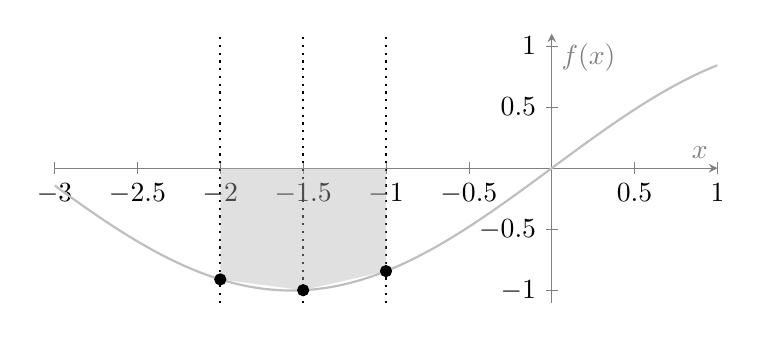
\begin{tikzpicture}
        \begin{axis}[
              width=10cm,
              height=5cm,
              axis x line=middle,
              axis y line=middle,
              xlabel={$x$},
              ylabel={$f(x)$},
              domain=-3:1,
              samples=100,
              ymin=-1.1, ymax=1.1,
              xmin=-3, xmax=1,
              legend style={at={(0.5,-0.2)},anchor=north},
              tick style={gray},
              label style={gray},
              axis line style={gray},
        ]
          % Vertical dotted lines at x=-2, -1.5, -1
          \addplot[dotted, thick, black, domain=-2:-2, samples=2] coordinates {(-2,-1.1) (-2,1.1)};
          \addplot[dotted, thick, black, domain=-1.5:-1.5, samples=2] coordinates {(-1.5,-1.1) (-1.5,1.1)};
          \addplot[dotted, thick, black, domain=-1:-1, samples=2] coordinates {(-1,-1.1) (-1,1.1)};
        % Continuous curve: sin(x) in light gray
        \addplot[gray!50, thick, smooth] {sin(deg(x))};
        % Trapezoids for intervals [-2,-1.5] and [-1.5,-1]
        \addplot [
            fill=gray!60, fill opacity=0.4, draw=none
        ] coordinates {
            (-2, -0.90930)
            (-1.5, -0.99749)
            (-1.5, 0)
            (-2, 0)
            (-2, -0.90930)
        };
        \addplot [
            fill=gray!60, fill opacity=0.4, draw=none
        ] coordinates {
            (-1.5, -0.99749)
            (-1, -0.84147)
            (-1, 0)
            (-1.5, 0)
            (-1.5, -0.99749)
        };
        % Endpoints
        \addplot[black, only marks, mark=*] coordinates {
            (-2, -0.90930)
            (-1.5, -0.99749)
            (-1, -0.84147)
        };
        \end{axis}
    \end{tikzpicture}
    \caption{Continuous curve $f(x)=\sin(x)$ and trapezoid rule areas (gray trapezoids) for $a=-2$, $b=-1$, $h=0.5$. Black dots: endpoints. The area under the straight lines connecting endpoints illustrates the trapezoid rule approximation.}
    \label{fig:trapezoidrule}
\end{figure}


\newthought{Composite Trapezoid Rule} again applies the trapezoid rule to each subinterval and sums the results.
\begin{align*}
    \int_a^b f(x)\, dx &\approx \sum_{i=0}^{n-1} \int_{x_i}^{x_{i+1}} f(x)\, dx \\
    &\approx \sum_{i=0}^{n-1} \frac{h}{2} \left[ f(x_i) + f(x_{i+1}) \right] \\
    &= \frac{h}{2} \left( f(x_0) + f(x_1) \right) + \frac{h}{2} \left( f(x_1) + f(x_2) \right) + \cdots + \frac{h}{2} \left( f(x_{n-1}) + f(x_n) \right) \\
    &= \frac{h}{2} \left[ f(x_0) + 2f(x_1) + 2f(x_2) + \cdots + 2f(x_{n-1}) + f(x_n) \right] \\
    &= \frac{h}{2} \left[ f(a) + 2\sum_{i=1}^{n-1} f(x_i) + f(b) \right]
\end{align*}
where $x_i = a + i h$ for $i = 0, 1, \ldots, n$.


The function values at the endpoints $a$ and $b$ are each weighted by $1$ in the formula, while all interior points are weighted by $2$. 
Intuitively, this is because each interior point contributes to two adjacent trapezoids, while the endpoints only contribute to one trapezoid each.
In your mind step through the circled enpoints in the figure above, and see how the interior points get counted twice, once as a right endpoint and once as a left endpoint, while the endpoints only get counted once.


\marginnote{\newthought{Dividing the integral by $h$} gives us a weighted average of the function values, which is a better approximation to the integral than just using the midpoint or endpoints. 
Implicitly reflecting local curvature and information about the function's behavior across the interval.}


\index{Simpson's rule}

\newthought{Simpson's rule} can capture curvature and thus often provides a much better approximation than the trapezoid rule.
Following the idea of fitting a linear function, we fit a quadratic polynomial through 3 points instead of a line through 2. 
You will see Simpson's rule is exact for quadratic polynomials.



\begin{figure}[h]
    \centering
    % Requires: \usepackage{pgfplots}
    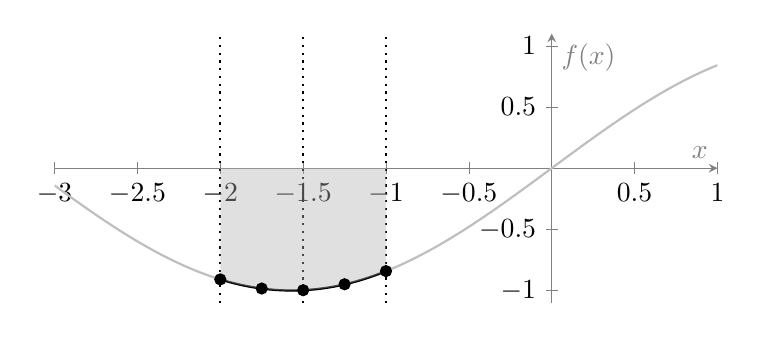
\begin{tikzpicture}
        \begin{axis}[
              width=10cm,
              height=5cm,
              axis x line=middle,
              axis y line=middle,
              xlabel={$x$},
              ylabel={$f(x)$},
              domain=-3:1,
              samples=100,
              ymin=-1.1, ymax=1.1,
              xmin=-3, xmax=1,
              legend style={at={(0.5,-0.2)},anchor=north},
              tick style={gray},
              label style={gray},
              axis line style={gray},
        ]
          % Vertical dotted lines at x=-2, -1.5, -1
          \addplot[dotted, thick, black, domain=-2:-2, samples=2] coordinates {(-2,-1.1) (-2,1.1)};
          \addplot[dotted, thick, black, domain=-1.5:-1.5, samples=2] coordinates {(-1.5,-1.1) (-1.5,1.1)};
          \addplot[dotted, thick, black, domain=-1:-1, samples=2] coordinates {(-1,-1.1) (-1,1.1)};
        % Continuous curve: sin(x) in light gray
        \addplot[gray!50, thick, smooth] {sin(deg(x))};
        % Simpson's rule: quadratic interpolant for [-2, -1.5, -1]
        \addplot[
            black,
            thick,
            domain=-2:-1,
            samples=50,
        ] {(-0.90930)*((x+1.5)*(x+1))/0.5 + (-0.99749)*((x+2)*(x+1))/(-0.25) + (-0.84147)*((x+2)*(x+1.5))/0.5};
        % Fill under the parabola for Simpson's rule on [-2, -1]
        \addplot [
            fill=gray!60, fill opacity=0.4, draw=none,
            domain=-2:-1,
            samples=50
        ] {(-0.90930)*((x+1.5)*(x+1))/0.5 + (-0.99749)*((x+2)*(x+1))/(-0.25) + (-0.84147)*((x+2)*(x+1.5))/0.5} \closedcycle;
        % Endpoints for [-2, -1.5, -1]
        \addplot[black, only marks, mark=*] coordinates {
            (-2, -0.90930)
            (-1.5, -0.99749)
            (-1, -0.84147)
        };
        % Midpoints for Simpson's rule intervals
        \addplot[black, only marks, mark=*] coordinates {
            (-1.75, -0.98363)
            (-1.25, -0.94898)
        };
        \end{axis}
    \end{tikzpicture}
    \caption{Continuous curve $f(x)=\sin(x)$ and Simpson's rule areas (gray, under the parabolas) for $a=-2$, $b=-1.5$, $h=0.5$ and $a=-1.5$, $b=-1$, $h=0.5$. 
    Black dots: endpoints. Black dots: midpoints at $x=-1.75$ and $x=-1.25$. Solid line at $x=-1.5$ separates the two intervals. 
    Each parabola illustrates the quadratic interpolant used by Simpson's rule on its subinterval.}
    \label{fig:simpsonrule}
\end{figure}

\newthought{Lagrange interpolation and quadrature.}
Lagrange interpolation constructs the unique polynomial of degree \(\le n\) that passes through given nodes $\{(x_j,y_j)\}_{j=0}^n$ using the basis
\begin{equation}
L_j(x)=\prod_{\substack{m=0 \\ m\neq j}}^{n} \frac{x - x_m}{x_j - x_m}.
\end{equation}

The general form of a quadratic polynomial is:
\begin{align*}
    f(x) = f(a) \cdot \frac{(x-m)(x-b)}{(a-m)(a-b)} + f(m) \cdot \frac{(x-a)(x-b)}{(m-a)(m-b)} + f(b) \cdot \frac{(x-a)(x-m)}{(b-a)(b-m)}
\end{align*}
\marginnote{\newthought{Try with some points.} Start with $x=0$ and see how the linear factors play out.}


For a symmetric interval, the area under $f(x)$ is best approximated by giving the endpoints weight $h/6$ each and the midpoint weight $2h/3$:
$A = C = h/6$, $B = 2h/3$ - we can verify this by integrating the Lagrange basis polynomials over $[a, b]$ 
and confirming that they yield these weights, but we omit the detailed calculation here.
In a symmetric interval, the nodes are equally spaced: \(x_0=a\), \(x_1=m=\tfrac{a+b}{2}\), \(x_2=b\), so that the midpoint satisfies \(m-a=b-m=h\).

Thus,
\begin{align*}
    \int_a^b f(x) \, dx &\approx \frac{h}{6} f(a) + \frac{2h}{3} f(m) + \frac{h}{6} f(b) \\
    &= \frac{h}{6} [f(a) + 4f(m) + f(b)]
\end{align*}

\newthought{Composite Simpson's Rule} again applies Simpson's rule on each pair of subintervals and 
sums the results (assume $n$ is even and $x_i=a+ih$). Starting from the integral:\\


\begin{align*}
    \int_a^b f(x)\, dx &\approx \sum_{i=0}^{n-1} \int_{x_i}^{x_{i+1}} f(x)\, dx \\
    &\approx \sum_{k=0}^{n/2-1} \frac{h}{6}\bigl[f(x_{2k}) + 4f(x_{2k+1}) + f(x_{2k+2})\bigr]\ \\
    &= \frac{h}{6}\Bigl[f(x_0) + 4\sum_{k=0}^{n/2-1} f(x_{2k+1}) + 2\sum_{k=1}^{n/2-1} f(x_{2k}) + f(x_n)\Bigr] \\
    &= \frac{h}{3}\left[f(x_0) + 4\sum_{\substack{i=1\\ i\ \text{odd}}}^{n-1} f(x_i) + 2\sum_{\substack{i=2\\ i\ \text{even}}}^{n-2} f(x_i) + f(x_n)\right].
\end{align*}
\marginnote{What happens, when you approximate a linear function with a quadratic?} 
\marginnote{\newthought{Runge's phenomenon:} High-degree polynomial interpolation oscillates due to overfitting, leading to large errors at the edges of the interval.}

\iffalse
\newthought{Quadrature rules in general}  
are formulas for approximating definite integrals by weighted sums of function values at specific points (nodes) in the interval. The general form is:
\begin{equation}
    \int_a^b f(x)\,dx \approx \sum_{i=1}^n w_i f(x_i)
\end{equation}
where $x_i$ are the nodes and $w_i$ are the weights. Different quadrature rules choose nodes and weights differently:
Gaussian quadrature is a powerful family of quadrature rules that chooses both the nodes $x_i$ and weights $w_i$ optimally (not equally spaced) to maximize accuracy. For $n$ nodes, Gaussian quadrature is exact for all polynomials up to degree $2n-1$. The most common case is Gauss-Legendre quadrature, which integrates functions on $[-1,1]$ using roots of Legendre polynomials as nodes. Unlike Newton-Cotes rules, Gaussian quadrature achieves much higher accuracy with fewer function evaluations, especially for smooth integrands.
\index{Legendre polynomials}
\newthought{Legendre polynomials} are a sequence of orthogonal polynomials $P_n(x)$ defined on the interval $[-1, 1]$. They satisfy the orthogonality relation:
\[
\int_{-1}^1 P_n(x) P_m(x) \, dx = 0 \quad \text{for } n \neq m
\]
and are solutions to Legendre's differential equation. The first few are:
\begin{align*}
P_0(x) &= 1 \\
P_1(x) &= x \\
P_2(x) &= \frac{1}{2}(3x^2 - 1) \\
P_3(x) &= \frac{1}{2}(5x^3 - 3x)
\end{align*}
In Gauss-Legendre quadrature, the nodes $x_i$ are chosen as the roots of $P_n(x)$.


\begin{equation}
    \int_a^b f(x) \, dx \approx \frac{h}{3}[f(a) + 4f(m) + f(b)]
\end{equation}

where $m = (a+b)/2$ and $h = (b-a)/2$.

\fi


\newthought{Practical advice:} Stop at Simpson. For higher accuracy, use composite rules with more subintervals. 
High-degrees ($n \geq 8$) develop negative weights and become unstable.


\begin{table*}[ht]
\centering
\begin{tabular*}{\textwidth}{@{\extracolsep{\fill}}p{0.33\textwidth}p{0.33\textwidth}p{0.33\textwidth}}
\toprule
\textbf{Method} & \textbf{Single Interval Error} & \textbf{Accumulated Error} \\
\midrule
Left/Right & $O(h^2)$ & $O(h)$ \\
Midpoint & $O(h^3)$ & $O(h^2)$ \\
Trapezoid & $O(h^3)$ & $O(h^2)$ \\
Simpson's 1/3 & $O(h^5)$ & $O(h^4)$ \\
In General (Gaussian Quadrature) & $O(h^{2n})$ & $O(h^{2n-1})$ \\
\bottomrule
\end{tabular*}
\vspace{2em}
\caption{Comparison of quadrature method accuracies. Higher-order methods achieve given accuracy with fewer function evaluations. 
$h$ is the step size, and $n$ is the number of evaluation points for Gaussian quadrature.}
\label{tab:quadrature_comparison}
\end{table*}


\section{Monte Carlo \& the Curse of Dimensionality}
\index{curse of dimensionality} \index{Monte Carlo}

\newthought{For $d$-dimensional integrals,} deterministic quadrature with $N$ points per dimension needs $N^d$ total points.
\marginnote{\newthought{A neural network with} $d = 10^6$ or 1 million parameters 
would need $(N)^{10^6}$ grid points. Even $N = 2$ gives $2^{10^6}$, a number with 300,000 digits.}
There is no way to do this, let alone iterate on it during iterative optimization.



\newthought{Random sampling} allows to estimate the integral without evaluating it on a full grid. 
The integral can be rewritten as an expectation:
\begin{equation}
    I = \int_\Omega f(\mathbf{x}) \, d\mathbf{x} = |\Omega| \cdot \mathbb{E}_{\mathbf{X} \sim \text{Uniform}(\Omega)}[f(\mathbf{X})].
\end{equation}
This identity means the definite integral equals the domain volume times the average value of $f$ under a uniform draw from $\Omega$. Practically this motivates a sampling estimator: draw points uniformly in $\Omega$, compute $f$ at those points, average the results, and multiply by $|\Omega|$ to estimate the integral.

\marginnote{\newthought{$\Omega$} is the domain of integration, and $|\Omega|$ is its length. For a 1D integral over $[a, b]$, we have $|\Omega| = b - a$. For higher dimensions, it's the product of the lengths of each dimension.}

\newthought{Monte Carlo uniform sampling} on $[-2,-1]$.\\
Let $X\sim\mathrm{Uniform}(-2,-1)$. Then \\


\begin{equation}
    I = \frac{|\Omega|}{N} \sum_{i=1}^{N} f(\mathbf{X}_i), \qquad \mathbf{X}_i \stackrel{\text{i.i.d.}}{\sim} \text{Uniform}(\Omega).
\end{equation}



\begin{figure}[h]
    \centering
    % Requires: \usepackage{pgfplots}
    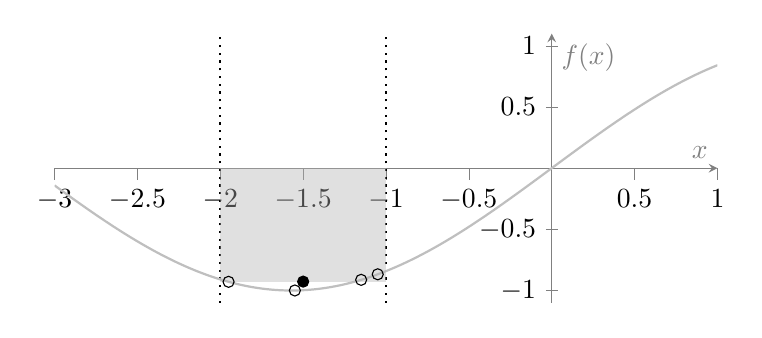
\begin{tikzpicture}
        \begin{axis}[
              width=10cm,
              height=5cm,
              axis x line=middle,
              axis y line=middle,
              xlabel={$x$},
              ylabel={$f(x)$},
              domain=-3:1,
              samples=100,
              ymin=-1.1, ymax=1.1,
              xmin=-3, xmax=1,
              legend style={at={(0.5,-0.2)},anchor=north},
              tick style={gray},
              label style={gray},
              axis line style={gray},
              ybar,
              bar width=0.5,
        ]
                % Vertical dotted guide lines (use axis coordinates to avoid interfering with plots)
                    \draw[dotted, thick, black] (axis cs:-2,-1.1) -- (axis cs:-2,1.1);
                    \draw[dotted, thick, black] (axis cs:-1,-1.1) -- (axis cs:-1,1.1);
        % Continuous curve: sin(x) in light gray
        \addplot[gray!50, thick, smooth] {sin(deg(x))};
        % Gray bar for single midpoint interval (average of MC samples)
        \addplot[ybar, bar width=1, fill=gray!60, fill opacity=0.4, draw=none] coordinates {
            (-1.5, -0.927228)
        };
        % Monte Carlo (random) samples shown as red dots (sample x in [-2,-1])
        \addplot[black, only marks, mark=o] coordinates {
            (-1.95, -0.92895)
            (-1.55, -0.99978)
            (-1.15, -0.91276)
            (-1.05, -0.86742)
        };
        % Average value of the samples shown as a black dot (single midpoint)
        \addplot[black, only marks, mark=*] coordinates {
            (-1.5, -0.927228)
        };
        \end{axis}
    \end{tikzpicture}
    \caption{Continuous curve $f(x)=\sin(x)$ and midpoint rule integrals (gray bars) for $a=-2$, $b=-1$, $h=0.5$. Circles: endpoints.
    The bars now touch, illustrating the midpoint rule without a gap.}
    \label{fig:montecarlo}
\end{figure}

\marginnote{\newthought{Midpoint rule} is a special case of Monte Carlo with $N=1$ sample at the midpoint.}

\newthought{Bias.} Because expectation is linear, this estimator is unbiased, meaning its expected value equals the true integral, for the number of $N \to \infty$:
\begin{equation}
    \mathbb{E}[\hat I_N] = I. 
\end{equation}

\marginnote{\newthought{i.i.d}, independent and identically distributed, means that all $\mathbf{X}_i$ are not correlated and that they all come from the same underlying distribution.}

\newthought{Variance.} The variance, a measure of the spread of the estimator around its mean, or how how large the error of the estimator can be,
follows from independence of the samples:
\begin{equation}
    \mathrm{Var}(\hat I_N) = \frac{|\Omega|^2}{N} \mathrm{Var}\bigl(f(\mathbf{X})\bigr) = \frac{|\Omega|^2 \sigma_f^2}{N},
\end{equation}

where $\sigma_f^2 = \mathrm{Var}(f(\mathbf{X}))$. Hence the standard error is

\begin{equation}
    \mathrm{SE}(\hat I_N) = \frac{|\Omega|\,\sigma_f}{\sqrt{N}}.
\end{equation}

% TODO: Make the break-even dimension between grid quadrature and Monte
% Carlo explicit. For a $d$-dimensional grid with $N$ total evaluations,
% the per-axis spacing is $h = N^{-1/d}$, so a second-order rule
% (midpoint, trapez) yields error $O(h^2) = O(N^{-2/d})$. Setting this
% equal to the Monte Carlo rate $O(N^{-1/2})$ gives $2/d = 1/2$, hence
% $d = 4$. Currently the chapter says only "MC is attractive in high
% dimensions" qualitatively; the concrete break-even at $d \approx 4$
% should be added (e.g. as a worked margin note here) so that exam
% questions asking for the crossover dimension are answerable purely
% from the script. Referenced by exam_01 2(c).
\newthought{Dimension independent.}
It is trivial to see, that for large $N$ the sampling error converges with, $O(1/\sqrt{N})$ for Monte Carlo, which makes it attractive in high dimensions.
Quadrature rules outperform in terms of their convergence rates, but the convergence effort explodes with the dimension, as we need $N^d$ points to maintain the same accuracy.

\begin{marginfigure}
    \centering
    \includegraphics[width=\marginparwidth]{figures/batchnoise.png}
    \caption{Effect of batch size on gradient noise: smaller batches produce larger variance 
    (showing up in the width of the training loss band) in the gradient estimate 
    (Source: \href{https://cs231n.github.io/neural-networks-3/\#baby}{Stanford CS231n Note}).}
    \label{fig:batchnoise}
\end{marginfigure}
\marginnote{As a beneficial side effect, computational cost is $n/b$ times cheaper per update step. 
For $n = 10^6$, and $b = 100$: SGD does 10,000 iterations with the compute GD needs for 1.}

\newthought{Convergence in SGD.} Mini-batch gradients used in SGD are Monte Carlo estimates of the true gradient, based on a samples drawn into a batch.
Increasing the batch size reduces variance roughly by $1/b$, directly analogous to the $1/N$ variance scaling above. 
This connection explains why batch size controls the noise–variance trade-off in training.



















% ==============================================================================================
% STUDENT ACTIVATION BLOCK

\newpage
\section{Examples \& Exercises}
\index{exercises}


\newthought{Let's stick} to our example from the methods sections, and calculate the integral of $\sin(x)$ from $-2$ to $-1$ 
using different methods. In order to be able to quantify the error of each method, we need the exact value. So let's compute the exact value of the integral:
\begin{align*}
        \tilde{I} &= \int_{-2}^{-1} \sin(x)\,dx \\
            &= [-\cos(x)]_{-2}^{-1} \\
            &= -\cos(-1) + \cos(-2) \\
            &\approx -0.9564491424.
\end{align*}

\newthought{Midpoint rule by hand.} Compute $\int_{-2}^{-1} \sin(x) dx$ using the midpoint rule with $n=1$ interval.
The midpoint is $m = (-2 + (-1))/2 = -1.5$, so the midpoint rule gives us:
\begin{align*}
    \hat{I} &\approx (b - a) \cdot f(m) \\
      &= 1 \cdot \sin(-1.5) \\
      &\approx -0.99749.
\end{align*}
The error is $|\tilde{I} - \hat{I}| \approx 0.04104$, which is the small difference between the midpoint estimate and the true value.

\marginnote{\newthought{Further things worth trying} are to calculate the approximation on the endpoints of the interval, comparing the error.}

\newthought{Midpoint rule with more intervals.} Now compute the midpoint rule with $n=2$ intervals, which means we will have two midpoints at $-1.75$ and $-1.25$.
This gives us: 
\begin{align*}
    h &= 0.5 \\
    \hat{I} &\approx h \cdot [f(-1.75) + f(-1.25)] \\
      &= 0.5 \cdot [\sin(-1.75) + \sin(-1.25)] \\
      &\approx -0.927228.
\end{align*}
The error is $|\tilde{I} - \hat{I}| \approx 0.02922$, which is smaller than the error with $n=1$ interval, illustrating how composites, or increasing the number of intervals improves the approximation.


\newthought{Trapezoid by hand.}
Use the trapezoid rule to compute $\int_{-2}^{-1} \sin(x) dx$ with $n=2$ intervals.
The endpoints are $-2$, $-1.5$, and $-1$. The trapezoid rule gives us:
\begin{align*}
    h &= 0.5 \\
    T_2 &= \frac{h}{2} [f(-2) + 2f(-1.5) + f(-1)] \\
        &= 0.25 \cdot [-0.90930 + 2(-0.99749) + (-0.84147)] \\
        &\approx -0.927228.
\end{align*}
The error is the same as the midpoint rule with $n=2$ intervals, which is not necessarily a coincidence, as both methods are second-order accurate and can yield similar results for certain functions and interval choices.




\vspace{2em}
\newthought{Simpson's rule by hand.} Use Simpson's rule to compute $\int_{-2}^{-1} \sin(x) dx$ with $n=2$ intervals.
The endpoints are $-2$, $-1.5$, and $-1$. Simpson's rule gives us:
\begin{align*}
    h &= 0.5 \\
    S_2 &= \frac{h}{3} [f(-2) + 4f(-1.5) + f(-1)] \\
        &= \frac{0.5}{3} \cdot [-0.90930 + 4(-0.99749) + (-0.84147)] \\
        &\approx -0.9564491424.
\end{align*}
The error is $|\tilde{I} - S_2| \approx 0.0000000000$, which is essentially zero, illustrating that Simpson's rule is exact for this particular integral, as $\sin(x)$ can be well approximated by a quadratic polynomial over the interval $[-2, -1]$.


\marginnote{\newthought{Try with more intervals,} see how the error decreases and check whether you know your way around composites in Simpson's and Trapezoid rules.}


\newthought{Monte Carlo by hand.} Use Monte Carlo estimation to compute $\int_{-2}^{-1} \sin(x) dx$ with $N=4$ random samples, 
which is similar to the compute efforts of the trapezoid method. Let's assume the random samples are: 
\begin{align*}
    X_1 &= -1.95, \quad f(X_1) = \sin(-1.95) \approx -0.92895, \\
    X_2 &= -1.55, \quad f(X_2) = \sin(-1.55) \approx -0.99978, \\
    X_3 &= -1.15, \quad f(X_3) = \sin(-1.15) \approx -0.91276, \\
    X_4 &= -1.05, \quad f(X_4) = \sin(-1.05) \approx -0.86742.
\end{align*}

The Monte Carlo estimate is:
\begin{align*}
    \hat{I} &= (b - a) \cdot \frac{1}{N} \sum_{i=1}^{N} f(X_i) \\
            &= 1 \cdot \frac{1}{4} (-0.92895 - 0.99978 - 0.91276 - 0.86742) \\
            &\approx -0.927228.
\end{align*}
The error is $|\tilde{I} - \hat{I}| \approx 0.02922$, which is the same as the midpoint method. 



\newthought{alternative error estimation for Monte Carlo.} For our concrete example with $N=4$ and the sample mean of
\(\bar f \approx -0.927228\). Using the unbiased sample variance estimator:
\begin{equation}
    Var(f(\mathbf{X})) = \frac{1}{N-1} \sum_{i=1}^N (f(X_i) - \bar f)^2.
\end{equation}

We obtain the sample variance and standard error of the Monte Carlo estimator as follows:
\begin{align*}
    \sigma_f^2 &= Var(f(\mathbf{X}))  \\ 
               &\approx 0.003036, \\
    \sigma_{f} &\approx 0.05512, \\
    \mathrm{SE}(\hat I_N) &\approx \frac{|\Omega|\, \sigma_f}{\sqrt{N}} \\
    &= \frac{1\cdot 0.05512}{2} \\
    &\approx 0.02756.
\end{align*}

What happens if we increase $N$ to 16? 
The error should decrease by a factor of 2, since the standard error scales as $1/\sqrt{N}$.
Briefly elaborate on how the error of the Monte Carlo estimator is dimension independant.






\vspace{2em}
\marginnote{\newthought{Code} can be found at \url{https://github.com/Quillstacks/lecturecode_numericalmethods.git}.}
\newthought{Enter higher dimensions on your machine.} Implement Monte Carlo integration for a $d$-dimensional integral, 
such as integrating a multivariate Gaussian function over a hypercube. While slowly increasing $d$, observe how the error behaves for different methods.
Even more, observe how grid-based quadrature methods become infeasible in terms of computational cost as $d$ grows.
Optionally, see how similar effects arise in optimization by implementing gradient descent and mini-batch
stochastic gradient descent on a high-dimensional function. Only watch compute times.


\vfill
\section{Self-Reflection and Recap}
\index{recap}

\newthought{Self-Reflection} Questions to guide your understanding:
\begin{itemize}
    \item How does the error of the midpoint, trapezoid, Simpson's rule and Monte Carlo compare?
    \item Why has the midpoint rule better accuracy than the left or right endpoint rules?
    \item How does composite methods improve accuracy, and what is the trade-off?
    \item Why do deterministic quadrature methods fail in high dimensions?
    \item In which way, is the midpoint rule a special case of Monte Carlo estimation?
    \item What is the intuition behind Monte Carlo not exploding in high dimensions?
    \item When would you use Simpson's rule vs.\ Monte Carlo?
    \item How is the mini-batch mean in SGD related to Monte Carlo estimation?
    \item How does the gradient estimation in SGD help escape local minima?
\end{itemize}

\newthought{Recap} of Key Concepts:
\begin{itemize}
    \item Deterministic quadrature methods (midpoint, trapezoid, Simpson's) approximate integrals using weighted sums of function values at 
    specific points. They are accurate and converge fast for smooth, low-dimensional problems.
    \item Monte Carlo integration estimates integrals by averaging function values at random samples. 
    It is unbiased and has a convergence rate of $O(1/\sqrt{N})$, making it independent of the dimensionality of the problem.
    \item In SGD, mini-batch gradients are Monte Carlo estimates of the true gradient.
\end{itemize}



\marginnote{\newthought{Teaser.} Are these six chapters really six things?}

\newthought{Six chapters in,} we have learned to represent numbers, reason about error,
find roots, optimize, integrate, and sample.
These felt like distinct topics.
In the next chapter, we will run them all once on one small dataset, and we will notice that they were facets of a single workflow all along: fitting a model to data.

%%%%%%%%%%%%%%%%%%%%%%%%%%%%%%%%%%%%%%%%%%%%%%%%%%%%%%%%%%%%%%%%%%%%%%%%%%%%%%

\index{Training}
\index{synthesis}
\index{neural network training}
\chapter{Training a Model from First Principles}
\printchapterversion{7_training_a_model}
\newthought{Oh, numerical methods are actually useful.}


% ==============================================================================================
% INTRODUCTION BLOCK

\section{The Why}
\index{training!motivation}


\newthought{The previous six chapters} developed numerical methdos.
These topics may appear distinct on a first reading,
but they share a wide-ranging application domain \cite{karpathy2019recipe}.


\index{chocolate}
\index{Nobel laureates}
\index{spurious correlation}

\newthought{The running dataset} for this chapter consists of fourteen countries with two associated quantities:
Per-capita chocolate consumption and Nobel laureates per ten million inhabitants \cite{messerlichocolate}.



\iffalse
\begin{table}[h]
\centering
\begin{tabular}{lrr}
\toprule
\textbf{Country} & \textbf{Chocolate} & \textbf{Nobel} \\
                 & (kg/person)        & (per 10M)      \\
\midrule
Switzerland    & 11.9 & 32 \\
Sweden         & 6.4  & 33 \\
Germany        & 11.6 & 13 \\
France         & 6.7  & 9  \\
United Kingdom & 9.5  & 21 \\
Norway         & 9.2  & 26 \\
Denmark        & 8.5  & 25 \\
Italy          & 4.0  & 4  \\
Netherlands    & 4.5  & 11 \\
Finland        & 7.3  & 7  \\
Austria        & 8.8  & 26 \\
Belgium        & 5.6  & 11 \\
United States  & 5.3  & 11 \\
Japan          & 1.8  & 2  \\
\bottomrule
\end{tabular}
\vspace{2em}
\caption{Per-capita chocolate consumption and Nobel laureates per ten million inhabitants.
Values are rounded and intended as a teaching dataset rather than as a research source.}
\label{tab:chocolate_data}
\end{table}
\fi


\newthought{The model} is a univariate linear regression of Nobel laureates on chocolate consumption (Figure~\ref{fig:chocolate_nobel_scatter}), fit by gradient descent on the mean squared error. The five correspondences below are illustrated against this model and dataset.


\begin{figure}[h]
    \centering
    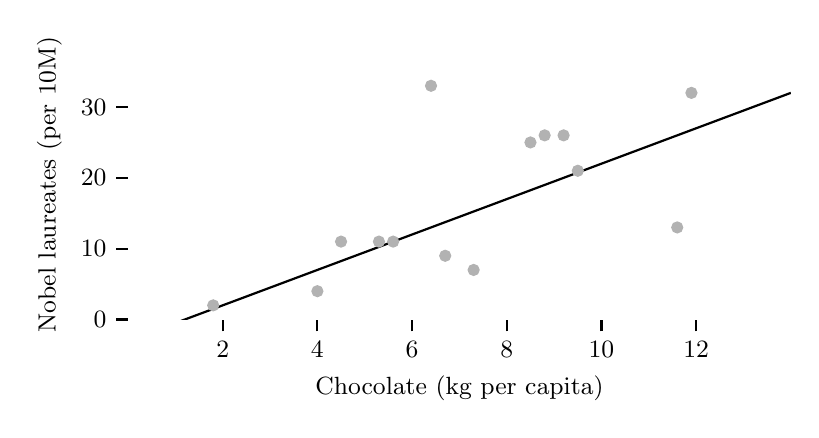
\begin{tikzpicture}
        \begin{axis}[
            width=10cm,
            height=5cm,
            xlabel={Chocolate (kg per capita)},
            ylabel={Nobel laureates (per 10M)},
            xmin=0, xmax=14,
            ymin=0, ymax=38,
            axis line style={draw=none},
            tick style={black, thick},
            xtick={2, 4, 6, 8, 10, 12},
            ytick={0, 10, 20, 30},
            xticklabel style={font=\small},
            yticklabel style={font=\small},
            tick align=outside,
            tick pos=left,
            label style={font=\small},
        ]
        \addplot[only marks, mark=*, mark size=2pt, gray!60] coordinates {
            (11.9, 32) (6.4, 33) (11.6, 13) (6.7, 9) (9.5, 21)
            (9.2, 26) (8.5, 25) (4.0, 4) (4.5, 11) (7.3, 7)
            (8.8, 26) (5.6, 11) (5.3, 11) (1.8, 2)
        };
        \addplot[black, thick, domain=0:14] {2.5*x - 3};
        \end{axis}
    \end{tikzpicture}
    \vspace{1em}
    \caption{The dataset and an approximate by-eye fit.
    The fit computed by gradient descent will not differ substantially.
    The Messerli correlation is real but spurious; chocolate consumption does not cause Nobel prizes, and plausible confounders include per-capita wealth and education.}
    \label{fig:chocolate_nobel_scatter}
\end{figure}


\marginnote{\newthought{Model}\\
$\hat{y}(x) = w x + b$.}

\marginnote{\newthought{Loss}\\
$L(w, b) = \tfrac{1}{n} \sum_{i=1}^{n} ( w x_i + b - y_i )^2$.}


\newthought{The Learning Objectives} are:
Identify numerical method in application, apply standard numerical methods in practical contexts, and finally think in frameworks.





% ==============================================================================================
% MAIN MIRRORS BLOCK

\newpage
\section{Overfitting as a Sanity Check}
\index{overfit single batch}
\index{Lagrange interpolation!model capacity}
\index{Newton method!sanity check}

\marginnote{\newthought{Recall Chapter 4.}
Newton's method converges in a single step from any starting point when applied to a quadratic function,
because the linear approximation of the derivative is exact in that case.}

\newthought{A standard recommendation in training} is to verify,
that the model can drive the loss to approximately zero on a small subset of the training data.
A failure to achieve this condition indicates an error in the model definition,
the loss formulation,
or the data pipeline.


\newthought{An example calculation} demonstrates the principle on a stripped down version of the dataset.
Pick just two countries, Italy at $(4.0, 4)$ and the United Kingdom at $(9.5, 21)$,
and extend the model by adding parameters,
\begin{align*}
    \hat{y}(x) = w_0 + w_1 x + w_2 x^2 + w_3 x^3 + w_4 x^4,
\end{align*}
with $n = 4$ here, giving five free parameters for only two training points.
The system is underdetermined:
infinitely many parameter settings drive the training loss to zero,
since any function passing through both training points qualifies.
A correctly implemented training loop on this overparameterized model must 
reach one of these zero-loss solutions (within machine precision).
Figure~\ref{fig:overfit_polynomial} shows one such solution:

\begin{figure}[h]
    \centering
    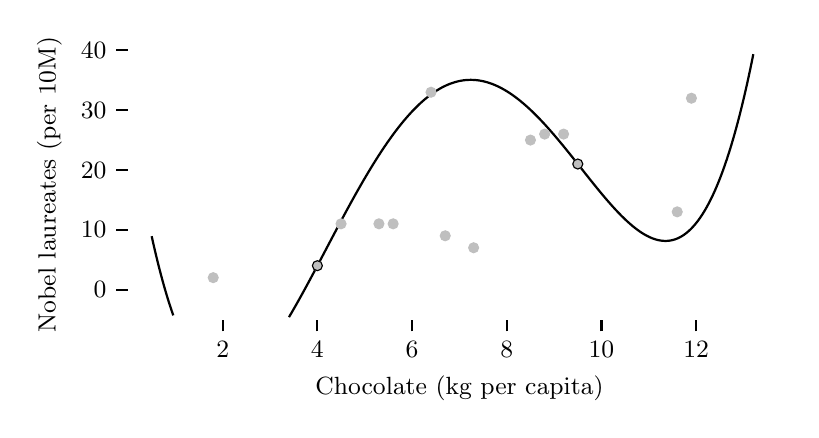
\begin{tikzpicture}
        \begin{axis}[
            width=10cm,
            height=5cm,
            xlabel={Chocolate (kg per capita)},
            ylabel={Nobel laureates (per 10M)},
            xmin=0, xmax=14,
            ymin=-5, ymax=40,
            restrict y to domain=-5:40,
            unbounded coords=jump,
            samples=400,
            axis line style={draw=none},
            tick style={black, thick},
            xtick={2, 4, 6, 8, 10, 12},
            ytick={0, 10, 20, 30, 40},
            xticklabel style={font=\small},
            yticklabel style={font=\small},
            tick align=outside,
            tick pos=left,
            label style={font=\small},
        ]
        \addplot[only marks, mark=*, mark size=1.8pt, gray!50] coordinates {
            (11.9, 32) (6.4, 33) (11.6, 13) (6.7, 9) (9.5, 21)
            (9.2, 26) (8.5, 25) (4.0, 4) (4.5, 11) (7.3, 7)
            (8.8, 26) (5.6, 11) (5.3, 11) (1.8, 2)
        };
        \addplot[black, thick, domain=0.5:13.5] {
            3.0909*x - 8.3636 + 0.08*(x-1)*(x-4)*(x-9.5)*(x-13)
        };
        \addplot[only marks, mark=o, mark size=1.8pt, black] coordinates {
            (4.0, 4) (9.5, 21)
        };
        \end{axis}
    \end{tikzpicture}
    \caption{Two training points (circled gray dots) selected from the dataset.
    Any function through both points is a zero-loss solution.
    It interpolates the two training points exactly but oscillates elsewhere,
    a textbook illustration of overfit capacity.}
    \label{fig:overfit_polynomial}
\end{figure}

\newthought{The sanity-check principle.}
The recommendation to drive the loss to zero on an overparameterized setup, where optimization is easy to achieve,
is the machine-learning instance of testing a solver on a problem with a known exact solution.

\vfill
\newthought{This separates the question of whether the implementation is correct
from the question of whether the method is suitable for the problem at hand.}

\marginnote{\newthought{Question.}
Figure~\ref{fig:overfit_polynomial} draws one zero-loss curve through the two training points.
How many such curves exist?
And what does that count imply about the geometry of the loss landscape this optimizer is asked to navigate? 
Welcome to the multiverse of global optima.}








\newpage
\section{Loss at Initialization}
\index{initialization!loss check}
\index{baseline test}

\marginnote{\newthought{Recall Chapter 4.}
A standard check for an iterative method, such as Newton's Method or SGD is to evaluate it at a configuration whose answer can be computed by hand.}

\newthought{A standard recommendation in training} is to inspect the loss before any optimization step has been taken.
The expected initial value follows from the data statistics and the chosen initialization;
a substantially different observed value points to a bug in the loss, the data, or the initialization.

\marginnote{\newthought{Classifier baseline.}
For a $K$-class classifier initialized to uniform output over the classes,
cross-entropy at step zero is $\log K$:
$\log 2 \approx 0.69$ for binary,
$\log 10 \approx 2.30$ for ten-way.
The first printed value is fixed by the architecture choice, not by the data.}

\newthought{An example calculation} on the chocolate dataset proceeds directly.
Initializing the regression with $w = 0$ and $b = \bar{y}$ makes the model predict $\bar{y}$ for every input,
so the mean squared error collapses to the mean squared deviation of the targets from their mean,
that is the empirical variance of the targets in the $1/n$ convention.
With $\bar{y} = 231/14 = 16.5$ and squared deviations summing to $1401.5$,
\begin{align*}
    L(0, \bar{y}) &= \frac{1}{n} \sum_{i=1}^{n} (y_i - \bar{y})^2 \\
                  &= \operatorname{Var}(y) \\
                  &\approx 100.1.
\end{align*}
A correct training loop therefore prints approximately $100$ as its first loss value.
A value of $5\,000$ indicates a summed rather than averaged loss;
a value of $0.0001$ indicates an unintended normalization;
a value far from $100$ in either direction indicates that the bias was not educatedly initialized (Figure~\ref{fig:init_loss}).


\begin{figure}[h]
    \centering
    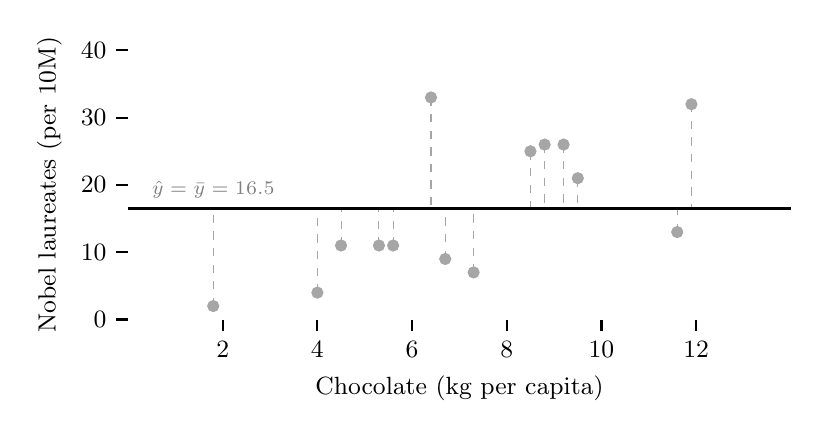
\begin{tikzpicture}
        \begin{axis}[
            width=10cm,
            height=5cm,
            xlabel={Chocolate (kg per capita)},
            ylabel={Nobel laureates (per 10M)},
            xmin=0, xmax=14,
            ymin=0, ymax=40,
            axis line style={draw=none},
            tick style={black, thick},
            xtick={2, 4, 6, 8, 10, 12},
            ytick={0, 10, 20, 30, 40},
            xticklabel style={font=\small},
            yticklabel style={font=\small},
            tick align=outside,
            tick pos=left,
            label style={font=\small},
        ]
        \addplot[gray!70, thin, dashed] coordinates {(1.8, 2) (1.8, 16.5)};
        \addplot[gray!70, thin, dashed] coordinates {(4.0, 4) (4.0, 16.5)};
        \addplot[gray!70, thin, dashed] coordinates {(4.5, 11) (4.5, 16.5)};
        \addplot[gray!70, thin, dashed] coordinates {(5.3, 11) (5.3, 16.5)};
        \addplot[gray!70, thin, dashed] coordinates {(5.6, 11) (5.6, 16.5)};
        \addplot[gray!70, thin, dashed] coordinates {(6.4, 33) (6.4, 16.5)};
        \addplot[gray!70, thin, dashed] coordinates {(6.7, 9) (6.7, 16.5)};
        \addplot[gray!70, thin, dashed] coordinates {(7.3, 7) (7.3, 16.5)};
        \addplot[gray!70, thin, dashed] coordinates {(8.5, 25) (8.5, 16.5)};
        \addplot[gray!70, thin, dashed] coordinates {(8.8, 26) (8.8, 16.5)};
        \addplot[gray!70, thin, dashed] coordinates {(9.2, 26) (9.2, 16.5)};
        \addplot[gray!70, thin, dashed] coordinates {(9.5, 21) (9.5, 16.5)};
        \addplot[gray!70, thin, dashed] coordinates {(11.6, 13) (11.6, 16.5)};
        \addplot[gray!70, thin, dashed] coordinates {(11.9, 32) (11.9, 16.5)};
        \addplot[black, thick, domain=0:14] {16.5};
        \addplot[only marks, mark=*, mark size=2pt, gray!70] coordinates {
            (11.9, 32) (6.4, 33) (11.6, 13) (6.7, 9) (9.5, 21)
            (9.2, 26) (8.5, 25) (4.0, 4) (4.5, 11) (7.3, 7)
            (8.8, 26) (5.6, 11) (5.3, 11) (1.8, 2)
        };
        \node[anchor=south west, font=\scriptsize, text=gray] at (axis cs:0.3, 16.5) {$\hat{y} = \bar{y} = 16.5$};
        \end{axis}
    \end{tikzpicture}
    \caption{Initialization with $w = 0$ and $b = \bar{y}$ predicts the constant $\bar{y} = 16.5$ for every input (horizontal line).
    The vertical segments are the residuals $y_i - \bar{y}$;
    the mean of their squares is the initial loss, $\operatorname{Var}(y) \approx 100$.}
    \label{fig:init_loss}
\end{figure}


\newthought{The boundary-value principle.}
A hand-computable value at a known starting configuration is the universal first verification step for any numerical procedure;
inspecting the initial loss against the variance of the targets is one instance.
It separates a failure of implementation, visible at step zero, from a failure of optimization, which can only show up after the first step is taken.






\newpage
\section{Mini-Batch Stochastic Gradient Descent}
\index{stochastic gradient descent}
\index{Monte Carlo!gradient}

\marginnote{\newthought{Curse of Dimensionality}
Monte Carlo integration averages the integrand at random samples and has standard error $1/\sqrt{N}$ independently of the dimension of the domain.
That dimension independence is what distinguishes it from grid quadrature, whose cost grows exponentially.}


\newthought{There is sample $x_n$ and feature dimension $d$,} use mini-batch stochastic gradient descent in place of 
full-batch gradient descent when dealing with data at scale.
At each iteration the gradient is estimated from a small random subset 
of the training data rather than from the entire dataset.
The loss is an expectation,
\begin{align*}
    L(\theta) = \mathbb{E}_{x \sim p_{\text{data}}} \big[ \ell(x; \theta) \big],
\end{align*}
and so is its gradient.
This substitution is not new.
The secant method in Chapter 4 replaced the exact derivative with a two-point finite-difference estimate,
and Newton's method replaced the objective with a truncated Taylor expansion.
Mini-batch stochastic gradient descent applies the same pattern on the data axis.

\newthought{An example calculation} on the chocolate dataset makes the variance visible.
Two mini-batches of size $B = 2$ are drawn from the fourteen countries; each yields the line through its two points,
\begin{align*}
    \hat{y}_P &= 3.54 x - 10.18, \\
    \hat{y}_Q &= -1.43 x + 17.43.
\end{align*}
The approximated gradient is the delta between the mini-batch line and the current overall approximation,
so each mini-batch supplies its own estimate of the same update direction,
and the spread of those deltas quantifies the variance of the stochastic estimator.

\begin{figure}[h]
    \centering
    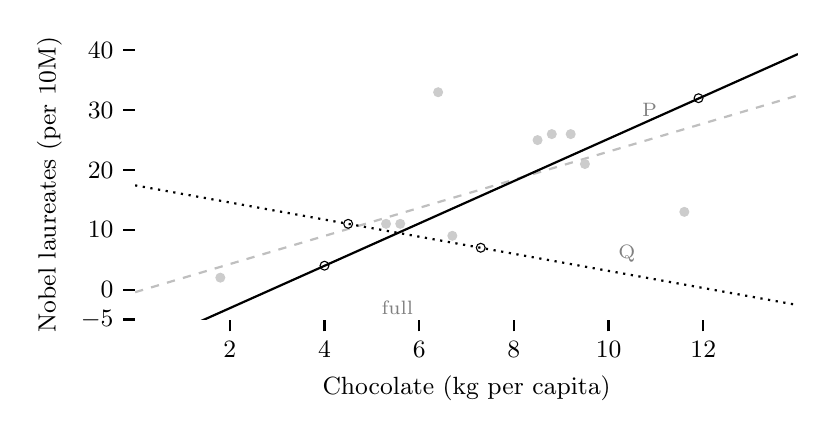
\begin{tikzpicture}
        \begin{axis}[
            width=10cm,
            height=5cm,
            xlabel={Chocolate (kg per capita)},
            ylabel={Nobel laureates (per 10M)},
            xmin=0, xmax=14,
            ymin=-5, ymax=40,
            axis line style={draw=none},
            tick style={black, thick},
            xtick={2, 4, 6, 8, 10, 12},
            ytick={-5, 0, 10, 20, 30, 40},
            xticklabel style={font=\small},
            yticklabel style={font=\small},
            tick align=outside,
            tick pos=left,
            label style={font=\small},
        ]
        % Full-batch reference fit
        \addplot[gray!50, thick, dashed, domain=0:14] {2.35*x - 0.43};
        % Mini-batch fits
        \addplot[black, thick, domain=0:14] {3.54*x - 10.18};
        \addplot[black, thick, dotted, domain=0:14] {-1.43*x + 17.43};
        % Unused data points (grayed out)
        \addplot[only marks, mark=*, mark size=1.6pt, gray!40] coordinates {
            (6.4, 33) (11.6, 13) (6.7, 9) (9.5, 21) (9.2, 26)
            (8.5, 25) (8.8, 26) (5.6, 11) (5.3, 11) (1.8, 2)
        };
        % Mini-batch A points (used for solid fit)
        \addplot[only marks, mark=o, mark size=1.6pt, black] coordinates {
            (4.0, 4) (11.9, 32)
        };
        % Mini-batch B points (used for dotted fit)
        \addplot[only marks, mark=o, mark size=1.6pt, black] coordinates {
            (4.5, 11) (7.3, 7)
        };
        \node[anchor=west, font=\scriptsize, text=gray] at (axis cs:10.5, 30) {P};
        \node[anchor=west, font=\scriptsize, text=gray] at (axis cs:10, 6) {Q};
        \node[anchor=west, font=\scriptsize, text=gray] at (axis cs:5, -3) {full};
        \end{axis}
    \end{tikzpicture}
    \caption{Two mini-batch fits to the chocolate dataset,
    each passing through its two sampled countries (P solid, Q dotted),
    together with the current overall approximation (gray dashed).
    Open circles mark the points used by each fit; the remaining countries are grayed out.
    The approximated gradient is the delta between a mini-batch line and the current overall approximation.}
    \label{fig:minibatch_estimates}
\end{figure}

\vfill
\newthought{The stochastic-gradient principle.}
Mini-batch SGD is a moving target per step but not in expectation:
iterates fluctuate in a neighborhood of the minimum whose radius shrinks with the step size and with the batch.
The same noise that bars exact convergence dislodges iterates from shallow local minima where full-batch descent would settle.



\marginnote{\newthought{Question.}
For $n = 14$ a batch of $B = 4$ buys nothing; for $n = 10^9$ the full batch never fits in memory.
At which $n$ does the bottleneck flip with $1/\sqrt{B}$?}





\iffalse
\newpage
\section{The Shape of the Loss Curve}
\index{loss curve}
\index{conditioning!loss curve}
\index{neural network!loss landscape}

\marginnote{\newthought{Recall Chapter 3.}
The convergence rate of gradient descent on a quadratic loss is governed by the condition number $\kappa$.
The error after $n$ iterations contracts by a factor $\bigl((\kappa-1)/(\kappa+1)\bigr)^n$,
so small $\kappa$ converges rapidly and large $\kappa$ crawls.}

\newthought{A standard recommendation in training} is attentive inspection of the loss curve throughout the run.
The shape of the curve, not its final value alone, carries the diagnostic content.

\newthought{An example calculation} on the chocolate dataset makes the link concrete.
With a single normalized feature, the condition number is small, perhaps $\kappa \approx 5$,
and the contraction factor is
\begin{align*}
    \frac{\kappa - 1}{\kappa + 1} = \frac{4}{6} \approx 0.67,
\end{align*}
so each iteration shrinks the error to about two thirds of its previous value and the curve settles within a handful of steps.
Adding a second feature without rescaling, for instance per-capita GDP in single euros, sends $\kappa$ to the order of $10^{10}$, the contraction factor to essentially one, and the loss curve to apparent flatness for any practical duration of training.
Figure~\ref{fig:loss_curve_shape} contrasts the two regimes on a common axis.

\begin{figure}[h]
    \centering
    \begin{tikzpicture}
        \begin{axis}[
            width=10cm,
            height=5cm,
            xlabel={iteration $n$},
            ylabel={loss $L_n$},
            xmin=0, xmax=50,
            ymin=0.01, ymax=100,
            ymode=log,
            log basis y=10,
            axis line style={draw=none},
            tick style={black, thick},
            xtick={0, 10, 20, 30, 40, 50},
            ytick={0.01, 0.1, 1, 10, 100},
            xticklabel style={font=\small},
            yticklabel style={font=\small},
            tick align=outside,
            tick pos=left,
            label style={font=\small},
        ]
        \addplot[black, thick, samples=51, domain=0:50]
            {100 * ((5-1)/(5+1))^x};
        \addplot[black, thick, dashed, samples=51, domain=0:50]
            {100 * ((100-1)/(100+1))^x};
        \node[anchor=west, font=\scriptsize, text=gray] at (axis cs:11, 0.5) {$\kappa{=}5$};
        \node[anchor=west, font=\scriptsize, text=gray] at (axis cs:30, 40) {$\kappa{=}100$};
        \end{axis}
    \end{tikzpicture}
    \caption{Loss curves of gradient descent on the chocolate dataset under two conditioning regimes,
    log scale on the loss axis.
    The solid curve corresponds to a well-conditioned setup ($\kappa = 5$) and reaches near-zero loss within a handful of iterations.
    The dashed curve corresponds to an ill-conditioned setup ($\kappa = 100$) and crawls.
    The shape of the curve identifies the regime.}
    \label{fig:loss_curve_shape}
\end{figure}

\newthought{Neural networks complicate the picture but reuse the instinct.}
The high-dimensional non-convex landscape of a deep network has mostly saddle points rather than minima \cite{DeepLearningBookNumericalComputation},
so a long plateau may signal an ill-conditioned quadratic or a slow escape from a saddle, and a sharp drop may signal a cliff.
The vocabulary expands; reading the curve as the first diagnostic does not.

\newthought{The conditioning principle.}
The recommendation to read the loss curve and the numerical methods practice of inferring the condition number from a convergence rate are the same procedure.

\vfill
\newthought{This reuses one diagnostic instinct} across convex regression and non-convex deep learning alike.

\marginnote{\newthought{Question.}
If your loss curve is flat for one hundred steps, is your problem ill-conditioned, stuck at a saddle, or just plain broken?
And how would you tell the three apart with one more experiment?
The curve talks; the question is whether you listen.}




\newpage
\section{Random Hyperparameter Search}
\index{hyperparameter search}
\index{curse of dimensionality}
\index{Monte Carlo!hyperparameters}

\marginnote{\newthought{Recall Chapter 6.}
In a $d$-dimensional cube, a grid with $N$ points per axis requires $N^d$ evaluations.
Monte Carlo accuracy depends on the total number of samples, not on $d$,
so for any but the smallest $d$ random sampling outperforms grid evaluation.}

\newthought{Standard practice} is to tune hyperparameters by random sampling of the hyperparameter space rather than by exhaustive grid search.
Random search consistently finds better configurations within a given compute budget;
a grid search that still terminates on a non-trivial model signals either a very small search space or a misallocated budget.

\newthought{An example calculation} makes the cost comparison concrete.
Tuning $d$ hyperparameters with $N = 5$ values per axis costs $N^d = 5^d$ evaluations by grid:
five at $d = 1$, three thousand at $d = 5$, nearly ten million at $d = 10$.
The random-search budget required for a fixed target accuracy is constant in $d$, by the dimension independence of Monte Carlo.
Figure~\ref{fig:curse_hyperparam} contrasts the two curves on a log axis.

\begin{figure}[h]
    \centering
    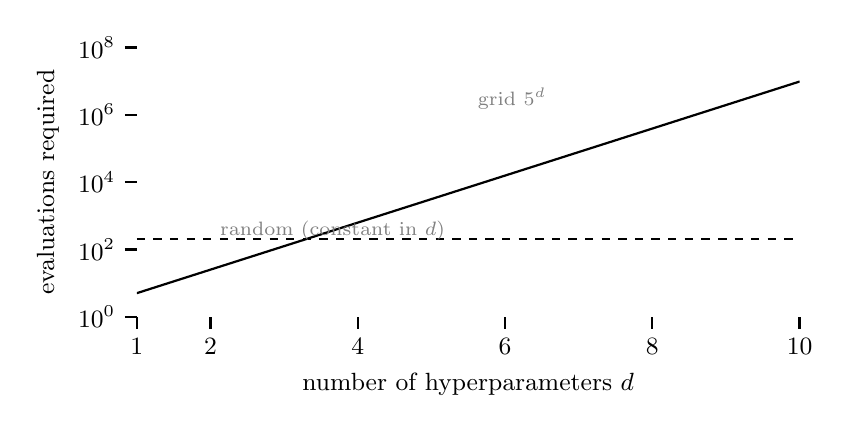
\begin{tikzpicture}
        \begin{axis}[
            width=10cm,
            height=5cm,
            xlabel={number of hyperparameters $d$},
            ylabel={evaluations required},
            xmin=1, xmax=10,
            ymin=1, ymax=1e8,
            ymode=log,
            log basis y=10,
            axis line style={draw=none},
            tick style={black, thick},
            xtick={1, 2, 4, 6, 8, 10},
            ytick={1, 100, 10000, 1000000, 100000000},
            xticklabel style={font=\small},
            yticklabel style={font=\small},
            tick align=outside,
            tick pos=left,
            label style={font=\small},
        ]
        \addplot[black, thick, samples=10, domain=1:10] {5^x};
        \addplot[black, thick, dashed, samples=10, domain=1:10] {200};
        \node[anchor=west, font=\scriptsize, text=gray] at (axis cs:5.5, 3e6) {grid $5^d$};
        \node[anchor=west, font=\scriptsize, text=gray] at (axis cs:2, 350) {random (constant in $d$)};
        \end{axis}
    \end{tikzpicture}
    \caption{Evaluations required by grid search ($5^d$) versus random sampling for a fixed target accuracy,
    on log axes.
    The grid cost grows exponentially with $d$;
    the random-search budget does not.
    For more than a handful of hyperparameters,
    only the latter is realistic.}
    \label{fig:curse_hyperparam}
\end{figure}

\newthought{The dimension-independence principle.}
Mini-batch stochastic gradient descent applies Monte Carlo to the gradient integral;
random hyperparameter search applies Monte Carlo to the validation-loss landscape.
Both rely on the same property: accuracy that does not depend on $d$.

\vfill
\newthought{This reuses the same square-root bound} that justified mini-batch training one section ago, in a different ambient dimension.

\marginnote{\newthought{Question.}
You have a budget of two hundred runs and seven hyperparameters to tune.
Where does a grid land you, where does random search land you, and how many of those seven are you secretly hoping do not matter?
Choose your dimensions before they choose you.}


\fi

\newpage
\section{Training Multiple Random Seeds}
% TODO find a better function to showcase this.. also a local minima would be nice, so we see two curves in the marginnote figure.
% Uncommented because like this it is not really worth it.
\index{global optimization}
\index{random restarts}

\marginnote{\newthought{Recall Chapter 5.}
For a non-convex objective, gradient descent terminates at a local minimum that depends on the initial point.
An effective global-optimization strategy is random restarts.}

\newthought{Repeat} training from several random initializations 
of the model parameters. The variance across runs is diagnostic about the loss landscape, 
and the run with the lowest loss is the candidate global solution \cite{picard2021seed}. 

\newthought{Composing} the slope from two parameters, with a quadratic trick on $w$ to 
introduce a symmetry, gives a concrete example of the principle.
\begin{align*}
    \hat{y}(x) = w^2 x + b.
\end{align*}
with minima at $w \approx \pm 1.53$ ($L \approx 60$) and a saddle at $w = 0$ ($L \approx 100$).

\marginnote{\newthought{Which would not have hurt at all} to be fair.} 

\newthought{With} two random starts, shown as circles in Figure~\ref{fig:multiple_seeds}.
Both basins recover the same fit $\hat{y} = 2.34 x - 0.43$;
a single seed would have surfaced only one solution in the whole space.

\vspace{1.5em}



\begin{figure}[h]
    \centering
    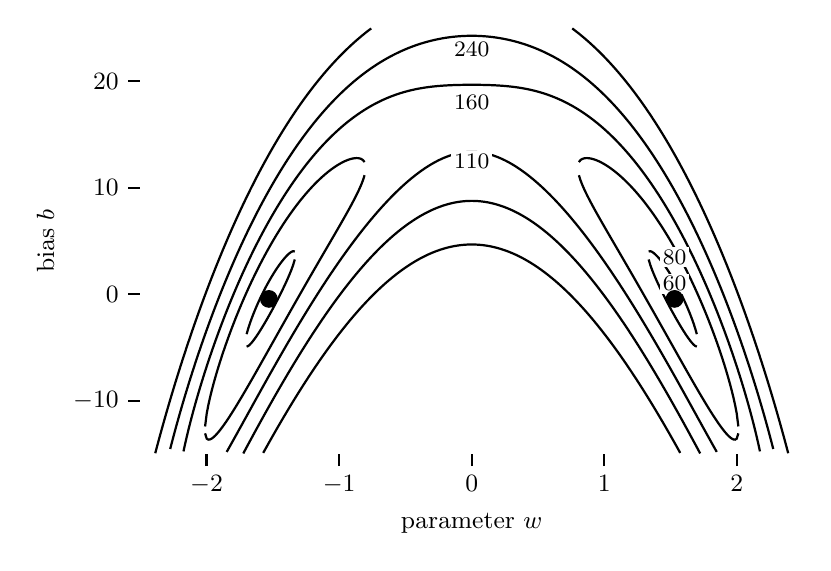
\begin{tikzpicture}
        \begin{axis}[
            width=10cm,
            height=7cm,
            xlabel={parameter $w$},
            ylabel={bias $b$},
            xmin=-2.5, xmax=2.5,
            ymin=-15, ymax=25,
            restrict y to domain=-15:25,
            unbounded coords=jump,
            axis line style={draw=none},
            tick style={black, thick},
            xtick={-2, -1, 0, 1, 2},
            ytick={-10, 0, 10, 20},
            xticklabel style={font=\small},
            yticklabel style={font=\small},
            tick align=outside,
            tick pos=left,
            label style={font=\small},
        ]
        \addplot[domain=-2.5:2.5, samples=400, thick, black]
          {(60 - 7.773*x^4 + 36.44*x^2 - 100.107 > 0) ? 16.5 - 7.221*x^2 + sqrt(60 - 7.773*x^4 + 36.44*x^2 - 100.107) : 1000};
        \addplot[domain=-2.5:2.5, samples=400, thick, black]
          {(60 - 7.773*x^4 + 36.44*x^2 - 100.107 > 0) ? 16.5 - 7.221*x^2 - sqrt(60 - 7.773*x^4 + 36.44*x^2 - 100.107) : 1000};
        \addplot[domain=-2.5:2.5, samples=400, thick, black]
          {(80 - 7.773*x^4 + 36.44*x^2 - 100.107 > 0) ? 16.5 - 7.221*x^2 + sqrt(80 - 7.773*x^4 + 36.44*x^2 - 100.107) : 1000};
        \addplot[domain=-2.5:2.5, samples=400, thick, black]
          {(80 - 7.773*x^4 + 36.44*x^2 - 100.107 > 0) ? 16.5 - 7.221*x^2 - sqrt(80 - 7.773*x^4 + 36.44*x^2 - 100.107) : 1000};
        \addplot[domain=-2.5:2.5, samples=400, thick, black]
          {(110 - 7.773*x^4 + 36.44*x^2 - 100.107 > 0) ? 16.5 - 7.221*x^2 + sqrt(110 - 7.773*x^4 + 36.44*x^2 - 100.107) : 1000};
        \addplot[domain=-2.5:2.5, samples=400, thick, black]
          {(110 - 7.773*x^4 + 36.44*x^2 - 100.107 > 0) ? 16.5 - 7.221*x^2 - sqrt(110 - 7.773*x^4 + 36.44*x^2 - 100.107) : 1000};
        \addplot[domain=-2.5:2.5, samples=400, thick, black]
          {(160 - 7.773*x^4 + 36.44*x^2 - 100.107 > 0) ? 16.5 - 7.221*x^2 + sqrt(160 - 7.773*x^4 + 36.44*x^2 - 100.107) : 1000};
        \addplot[domain=-2.5:2.5, samples=400, thick, black]
          {(160 - 7.773*x^4 + 36.44*x^2 - 100.107 > 0) ? 16.5 - 7.221*x^2 - sqrt(160 - 7.773*x^4 + 36.44*x^2 - 100.107) : 1000};
        \addplot[domain=-2.5:2.5, samples=400, thick, black]
          {(240 - 7.773*x^4 + 36.44*x^2 - 100.107 > 0) ? 16.5 - 7.221*x^2 + sqrt(240 - 7.773*x^4 + 36.44*x^2 - 100.107) : 1000};
        \addplot[domain=-2.5:2.5, samples=400, thick, black]
          {(240 - 7.773*x^4 + 36.44*x^2 - 100.107 > 0) ? 16.5 - 7.221*x^2 - sqrt(240 - 7.773*x^4 + 36.44*x^2 - 100.107) : 1000};
        \node[font=\footnotesize, fill=white, inner sep=1pt] at (axis cs:1.53, 1.0) {60};
        \node[font=\footnotesize, fill=white, inner sep=1pt] at (axis cs:1.53, 3.5) {80};
        \node[font=\footnotesize, fill=white, inner sep=1pt] at (axis cs:0, 12.5) {110};
        \node[font=\footnotesize, fill=white, inner sep=1pt] at (axis cs:0, 18) {160};
        \node[font=\footnotesize, fill=white, inner sep=1pt] at (axis cs:0, 23) {240};
        \addplot[only marks, mark=*, mark size=3pt, black]
            coordinates {(-1.53, -0.43) (1.53, -0.43)};
        \end{axis}
    \end{tikzpicture}
    \caption{Loss landscape $L(w, b)$ for $\hat{y}(x) = w^2 x + b$ on the chocolate data, drawn as iso-loss contours.
    Filled circles mark the two converged minima at $(w, b) = (\pm 1.53, -0.43)$ with $L \approx 57.4$,
    sitting on the curved valley $b^*(w) = 16.5 - 7.221\, w^2$. My wife also says it looks like the whale from 
    "Hitchhiker's Guide to the Galaxy". Okay, I added the book reference.}
    \label{fig:multiple_seeds}
\end{figure}

\iffalse
\begin{marginfigure}
    \centering
    \begin{tikzpicture}
        \begin{axis}[
            width=\marginparwidth,
            height=4cm,
            xlabel={Chocolate},
            ylabel={Nobel},
            xmin=0, xmax=14,
            ymin=0, ymax=38,
            axis line style={draw=none},
            tick style={black, thick},
            xtick={2, 6, 10},
            ytick={10, 20, 30},
            xticklabel style={font=\footnotesize},
            yticklabel style={font=\footnotesize},
            tick align=outside,
            tick pos=left,
            label style={font=\footnotesize},
        ]
        \addplot[only marks, mark=*, mark size=1.5pt, gray!60] coordinates {
            (11.9, 32) (6.4, 33) (11.6, 13) (6.7, 9) (9.5, 21)
            (9.2, 26) (8.5, 25) (4.0, 4) (4.5, 11) (7.3, 7)
            (8.8, 26) (5.6, 11) (5.3, 11) (1.8, 2)
        };
        \addplot[black, thick, domain=0:14] {1.53^2 * x - 0.43};
        \end{axis}
    \end{tikzpicture}
    \caption{Both minima of Figure~\ref{fig:multiple_seeds} produce the same fit $\hat{y} = 2.34\,x - 0.43$ on the chocolate data, since $w^2$ erases the sign of $w$.}
    \label{fig:multiple_seeds_fit}
\end{marginfigure}
\fi

\newthought{Cost Benefits}. Purely tuning the learning rate to chase variance that is actually 
basin-selection variance, is a common failure mode.

\newthought{Cost caveat.}
Multi-seed training multiplies compute by the number of seeds.
Routine at small-scale; at scale
the method only survives in partial-data form.
However, an empirical observation shows that,
distinct trained minima are typically joined by low-loss paths in parameter space as model-scale grows 
\cite{garipov2018modeconnectivity}.









\newpage
\section{Quantization for Inference}
\index{quantization}
\index{binary precision}

\marginnote{\newthought{Recall Chapter 2.}
Floating-point formats trade range against precision against bits.
The appropriate format for a given computation is the smallest one whose range and precision suffice.}

\newthought{The savings fall in two areas.}
At training time, parameters and gradients move less data through memory;
per-step throughput on bandwidth-bound hardware rises in proportion,
and even when low precision demands more steps to reach a comparable loss the product, 
operations until convergence, often remains favourable.
At inference the win compounds: floating-point multiplications collapse into cheap bitwise operations on dedicated hardware,
and a model whose parameters fit in cache stops paying the memory-latency tax that dominates inference for anything larger than the L2.

\begin{marginfigure}
    \centering
    \begin{tikzpicture}
        \begin{axis}[
            width=\marginparwidth,
            height=4cm,
            xlabel={bits per parameter},
            ylabel={loss},
            xmode=log,
            log basis x={2},
            xmin=0.7, xmax=45,
            ymin=6, ymax=15,
            axis line style={draw=none},
            tick style={black, thick},
            xtick={1, 8, 32},
            xticklabels={1, 8, 32},
            ytick={8, 10, 12, 14},
            xticklabel style={font=\footnotesize},
            yticklabel style={font=\footnotesize},
            tick align=outside,
            tick pos=left,
            label style={font=\footnotesize},
        ]
        \addplot[black, thick, mark=*, mark size=1.8pt] coordinates {
            (1, 13.3) (8, 7.9) (32, 7.6)
        };
        \end{axis}
    \end{tikzpicture}
    \caption{Loss against bits per parameter on the chocolate dataset.
    Binary precision pays a sharp penalty; the curve drops fast and flattens by integer precision.
    Most of the win sits in the first few bits.}
    \label{fig:precision_loss}
\end{marginfigure}

\newthought{An example calculation} on the chocolate model makes the trade visible.
Full-precision fitting, integer rounding to the nearest integer, and binary rounding 
to the nearest representative in $\{-1, +1\}$ produce three lines,
\begin{align*}
    &\hat{y}_{\text{full}}   = 2.35 x - 0.43, \\
    &\hat{y}_{\text{int}}    = 2 x, \\
    &\hat{y}_{\text{binary}} = x - 1.
\end{align*}
with root-mean-square errors
\begin{align*}
    &\text{L}_{\text{full}}   \approx 7.6, \\
    &\text{L}_{\text{int}}    \approx 7.9, \\
    &\text{L}_{\text{binary}} \approx 13.3,
\end{align*}




measured in Nobel laureates per ten million.
Figure~\ref{fig:binary_fit} overlays the three on the dataset.


\begin{figure}[h]
    \centering
    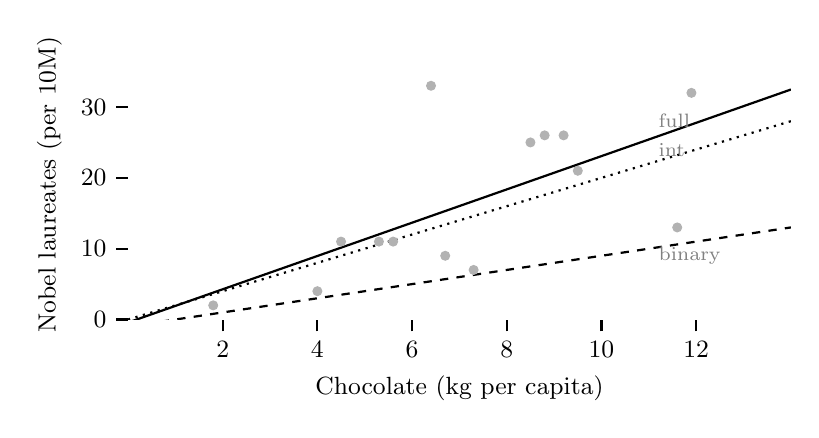
\begin{tikzpicture}
        \begin{axis}[
            width=10cm,
            height=5cm,
            xlabel={Chocolate (kg per capita)},
            ylabel={Nobel laureates (per 10M)},
            xmin=0, xmax=14,
            ymin=0, ymax=38,
            axis line style={draw=none},
            tick style={black, thick},
            xtick={2, 4, 6, 8, 10, 12},
            ytick={0, 10, 20, 30},
            xticklabel style={font=\small},
            yticklabel style={font=\small},
            tick align=outside,
            tick pos=left,
            label style={font=\small},
        ]
        \addplot[only marks, mark=*, mark size=1.6pt, gray!60] coordinates {
            (11.9, 32) (6.4, 33) (11.6, 13) (6.7, 9) (9.5, 21)
            (9.2, 26) (8.5, 25) (4.0, 4) (4.5, 11) (7.3, 7)
            (8.8, 26) (5.6, 11) (5.3, 11) (1.8, 2)
        };
        \addplot[black, thick, domain=0:14] {2.35*x - 0.43};
        \addplot[black, thick, dotted, domain=0:14] {2*x};
        \addplot[black, thick, dashed, domain=0:14] {x - 1};
        \node[anchor=west, font=\scriptsize, text=gray] at (axis cs:11, 28) {full};
        \node[anchor=west, font=\scriptsize, text=gray] at (axis cs:11, 24) {int};
        \node[anchor=west, font=\scriptsize, text=gray] at (axis cs:11, 9) {binary};
        \end{axis}
    \end{tikzpicture}
    \caption{Full-precision fit (solid), integer approximation $(w, b) = (2, 0)$ (dotted), and binary approximation $(w, b) = (+1, -1)$ (dashed) on the chocolate dataset.
    Integer rounding barely moves the root-mean-square error; binary near doubles it.}
    \label{fig:binary_fit}
\end{figure}


\vfill
\newthought{And another tradeoff,} where we give up precision and predictive performacnce, for runtime, memory and energy savings.

\marginnote{\newthought{Question.}
Integer precision matched the full-precision error on this dataset.
Why does any production model still ship in float32?
Where does the extra precision actually earn its bits, and where is it just inertia?}




% ==============================================================================================
% STUDENT ACTIVATION + RECAP BLOCK

\newpage
\section{Self-Reflection and Recap}
\index{recap}
\index{reflection}

\newthought{Self-Reflection} Questions to guide your understanding:
\begin{itemize}
    \item Why does driving the loss to zero on an overparameterized model detect bugs in the pipeline rather than in the optimizer?
    \item For the chocolate model initialized at $w = 0$, $b = \bar{y}$, the predicted first loss is $\operatorname{Var}(y) \approx 100$. What does a printed value of $5\,000$ tell you, and what does a printed value of $0.0001$ tell you?
    \item In what precise sense is mini-batch stochastic gradient descent a Monte Carlo estimator? What is being averaged, and over what?
    \item For the factored model $\hat{y}(x) = w^2 x + b$, why is the origin a saddle of the loss rather than a minimum, and what makes zero initialization a practical trap even so?
    \item Why can a model trained at higher precision be deployed at much lower precision without retraining, while training at the lower precision tends to fail?
\end{itemize}

\newthought{Recap} of Key Concepts:
\begin{itemize}
    \item Driving the loss to zero on an overparameterized model is the training version of testing a solver on a problem with a known exact answer.
    \item Inspecting the initial loss against the variance of the targets separates a failure of implementation, visible at step zero, from a failure of optimization, which can only appear after the first step.
    \item Mini-batch stochastic gradient descent is Monte Carlo applied to the gradient integral, with standard error $1/\sqrt{B}$ independent of the parameter dimension.
    \item Training from multiple random seeds is the random-restarts heuristic from Chapter 5 applied to a non-convex landscape; the seed picks the basin through the sign of the initial fluctuation at the origin saddle, and mini-batch noise supplies the annealing component implicitly.
    \item Quantization for inference is the precision-selection decision from Chapter 2 applied to a different computation: inference tolerates far less precision than training because it does not accumulate gradient updates, so the appropriate format is the smallest whose error budget is acceptable for the deployment.
\end{itemize}

\marginnote[2em]{\newthought{Outlook.} The same numerical methods (often) scale to billion-parameter models.
The cost and the engineering grow; the methods do not.}

\newthought{From numerical methods to modeling at scale.} The toolbox established in Chapters 1 to 6
is sufficient to describe the standard practices of model training at the scale of these notes.
At larger scales the parameter count grows by orders of magnitude and the data, too.
The engineering surrounding the training run grows correspondingly,
and the vocabulary drifts further from the language of classical numerical analysis.
None of this displaces the underlying methods.
The mechanics that decide whether a model's learning succeeds remain those introduced earlier.



% ==============================================================================================
% POTENTIAL ADD-ON MIRRORS (for future expansion; not currently in chapter)
%
% Each entry: Recipe recommendation  ↔  Corresponding numerical method (chapter)
% These correspondences were considered but not included, either because they
% require introducing material not yet covered in Chapters 1 to 6, or because
% they would lengthen the chapter past one correspondence per page.
%
% - Input-independent baseline (third Karpathy sanity-check step)
%       ↔ Degenerate input test for a numerical procedure (Ch3 + Ch6, quadrature
%         on a constant function should return constant times interval, etc.)
%
% - Weight decay
%       ↔ Tikhonov regularization for ill-conditioned inverse problems (Ch3,
%         would require introducing Tikhonov first)
%
% - Learning-rate schedules (cosine, warmup)
%       ↔ Adaptive step-size in iterative methods (Ch5, would need step-size
%         control as a new concept)
%
% - Adam and momentum-based optimizers
%       ↔ Heavy-ball and second-order methods (Ch4/Ch5, would need momentum
%         as a new concept)
%
% - Batch normalization
%       ↔ Per-layer preconditioning (Ch3, would need the depth-composition
%         argument that the chapter currently avoids)
%
% - Dropout
%       ↔ Random projection or ensemble of subsets (Ch6, would need a new
%         framing of dropout as Monte Carlo over sub-networks)
%
% - Early stopping
%       ↔ Truncation of an iterative method before machine precision is hit
%         (Ch4/Ch5, conceptually direct but pedagogically thin)
%
% - Gradient checkpointing
%       ↔ Space-time tradeoff in numerical computation (would need a separate
%         treatment of memory-compute tradeoffs)
%
% - Initial use of a default optimizer such as Adam
%       ↔ Use of the simplest sufficient method as a first choice (Ch5,
%         pedagogically thin)
%
% - Data augmentation
%       ↔ Importance sampling and variance reduction in Monte Carlo (Ch6,
%         would need importance sampling introduced first)
%
% - Mixed-precision training with loss scaling
%       ↔ Affine rescaling to keep values within the representable range
%         (Ch2, conceptually direct but adds a second Ch2 correspondence
%         beyond Correspondence 7)
%
% - Curriculum learning, easy-to-hard training
%       ↔ Homotopy and continuation methods in nonlinear solvers (would need
%         continuation as a new concept)
%
% ==============================================================================================

%%%%%%%%%%%%%%%%%%%%%%%%%%%%%%%%%%%%%%%%%%%%%%%%%%%%%%%%%%%%%%%%%%%%%%%%%%%%%%

%\input{chapters/8_quadrature.tex}             % extended: full Newton-Cotes, composite rules
%\input{chapters/9_romberg_montecarlo.tex}     % extended: Richardson, Romberg, variance reduction
%\input{chapters/10_interpolation.tex}
%\input{chapters/11_splines.tex}
%\input{chapters/12_fourier.tex}
%\input{chapters/13_odes.tex}
%\input{chapters/14_parallel_distributed.tex}
%\input{chapters/15_sgd_extended.tex}          % extended SGD: momentum, Adam, LR schedules



% Add index
% Check the code
% Think about printing this ones for myself. Learn how to make a bookcover. 
% Add a Probeklausur but in a separate latex document.  


\nocite{*}
\makestandardbackmatter{numerischemethoden}

\end{document}
